\documentclass[aspectratio=169]{beamer}

% Allow for any UTF8 input (accepts é, è, ö, ä, å, etc.)
\usepackage[utf8]{inputenc}
% Hyperref for links inside the document (at cite, ref, or others)
\usepackage{hyperref}

% Drawings with TikZ, what this tutorial is all about
% TikZ ist kein Zeichenprogramm - TikZ Is Not a Drawing Program
% Part of PGF (Portable Graphics Format)
\usepackage{tikz}
% Convenient TikZ libraries
% Calc for enabling mathematical operations between points
\usetikzlibrary{calc}
% Shapes for importing shapes to easily include in your drawing
\usetikzlibrary{shapes}
% More complex and tweakable arrow shapes (generally not needed)
\usetikzlibrary{arrows}
% Package with more TikZ symbols (generally not needed)
\usepackage{tikzsymbols}
% Package with TikZ symbols for drawing circuits (generally not needed)
\usepackage{circuitikz}
% 3D TikZ (generally not needed)
\usepackage{tikz-3dplot}

% PGFplots- Package to make it easier to plot things with TikZ
\usepackage{pgfplots}
% For subplots using PGFplots
\usepgfplotslibrary{groupplots}
% If including PGFplots, it is adviced to set the compatibility to a fixed version that works. For playing, use the newest.
\pgfplotsset{ compat = newest }

% Graphicx package for images
\usepackage{graphicx}

% My recommendation for tables and complex array structures in LaTeX
\usepackage{array}
% My recommendation for reference handling with bibtex files in beamer
\usepackage[backend=bibtex,doi=false,isbn=false,url=false,style=ieee]{biblatex}
\usepackage{bibentry}
\bibliography{papers}

% Title
\title{Practical TikZ tutorial}
% Author (avoiding PDF string problems)
\author{Pol del Aguila Pla \texorpdfstring{\\}{} Ph.D. candidate at the KTH Royal Institute of Technology \texorpdfstring{\\}{} \href{mailto://poldap@kth.se}{\texttt{poldap@kth.se}}, \href{https://people.kth.se/~poldap}{\texttt{people.kth.se/\texorpdfstring{$\sim$}{}poldap}} \texorpdfstring{\\}{}
\href{https://github.com/poldap/tikz-tutorial/fork}{Fork this tutorial on GitHub: github.com/poldap/tikz-tutorial}}
% Date
\date{January 2019}

\begin{document}

\maketitle

\begin{frame}{Motivating example - $0$ words introduction}
    
    \begin{itemize}
        \item The interest of a research topic in a simple animation. 
        \item Creativity and clear communication.
    \end{itemize}
    
    \begin{center}
		\begin{tikzpicture}
		    % My house
		    % A bed
			\node at (0,0) {\Bed[4]};
			% An oven
			\node at (8,0) {\oven[4]};
			% The walls of my home
			\draw (-1.4,-0.6) rectangle (9,2.5);
			% Draw a table
			\draw[thick] (5,-0.5) -- (5,0.4) -- (4.8,0.4) -- (4.8,0.6) -- (6.2,0.6) -- (6.2,0.4) -- (6,0.4) -- (6,-.5) -- (5.9,-.5) -- (5.9,00.4) -- (5.1,0.4) -- (5.1,-0.5) -- cycle;
			% Sleeping
			\only<1>{
			    \node at (-0.1,0.2) [rotate=90] {\Strichmaxerl[6][60][-60]};
			}
	    	% Waking up
			\only<2>{
			    \node at (1.5,0.2) {\Strichmaxerl[6][50][-50]};
			}
		    % On my way
			\only<3>{
			    \node at (2.5,0.2) {\Strichmaxerl[6][50][-50]};
				\node at (-.2,-.22) [txantenna]{};
			}
			% There
			\only<4->{
			    \only<4>{
				    \node at (3.5,0.2) {\Strichmaxerl[6][50][-50]};
				}
				\only<5>{
				    \node at (4.3,0.2) {\Strichmaxerl[6][50][-50]};
				}
				\only<6->{
				    \node at (4.3,0.2) {\Strichmaxerl[6][-45][45]};
				}
				\node at (8.4,.8) {\pot[1.8]};
				\node at (7.35,.8) {\fryingpan[2]};
				\node at (5,.78) {\Coffeecup[1]};
			}
			% Spies
			\only<7->{
			    \draw (11,-0.6) -- (9.5,-0.6) -- (9.5,2.5) -- (11,2.5);
				\node[red] at (10,0.2) {\Strichmaxerl[6]};
			}
			\end{tikzpicture} 
			\\
			The \only<7->{{\color{red} Privacy-Aware}} Internet of Things
	\end{center}
	\small Introduction to an old presentation - will not be published.
\end{frame}

\begin{frame}{Simply TikZ - ex.}

    \vspace{-30pt}
    
    % An example of the outcomes one can get from simple TikZ commands. Do not try to understand straight away, go first to the next slide, "Simply TikZ - Basics"
    \begin{center}
        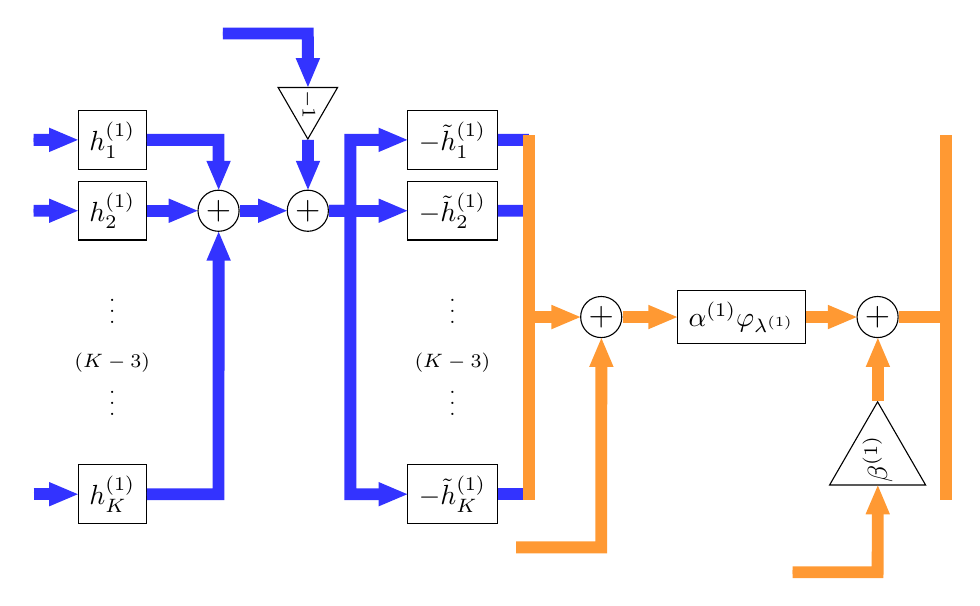
\begin{tikzpicture}[scale = 0.9,xscale = 1.2]
            % Define styles - Equivalent to repeating everything inside [] every time the style is used
            \tikzstyle{imagearrow} = [line width=.5mm,draw=blue!80!white,-triangle 45,postaction={draw, line width=1.5mm, shorten >=2mm, -}]
            \tikzstyle{imageline} = [line width=1.5mm,draw=blue!80!white,-];
            \tikzstyle{tensorarrow} = [line width=.5mm,draw=orange!80!white,-triangle 45,postaction={draw, line width=1.5mm, shorten >=2mm, -}]
            \tikzstyle{tensorline} = [line width=1.5mm,draw=orange!80!white,-];
            \tikzstyle{mult} = [isosceles triangle, draw, isosceles triangle apex angle=60, isosceles triangle stretches]
            % Nodes in the first hidden layer
            % Convolutional
            	% Direct operator
            	\node (c11) at (5,5) [draw,fill=white,shape=rectangle,inner sep = 4]{$h^{(1)}_1$};
            	\node (c12) at (5,4) [draw,fill=white,shape=rectangle,inner sep = 4]{$h^{(1)}_2$};
            	\node (c1dots) at (5,2) {\scriptsize$\begin{array}{c}\vdots\\\\(K-3)\\\vdots\end{array}$};
            	\node (c1K) at (5,0) [draw,fill=white,shape=rectangle,inner sep = 4]{$h^{(1)}_K$};
            	% Adjoint operator
            	\node (c11m) at (9,5) [draw,fill=white,shape=rectangle,inner sep = 4]{$-\tilde{h}^{(1)}_1$};
            	\node (c12m) at (9,4) [draw,fill=white,shape=rectangle,inner sep = 4]{$-\tilde{h}^{(1)}_2$};
            	\node (c1mdots) at (9,2) {\scriptsize$\begin{array}{c}\vdots\\\\(K-3)\\\vdots\end{array}$};
            	\node (c1Km) at (9,0) [draw,fill=white,shape=rectangle,inner sep = 4]{$-\tilde{h}^{(1)}_K$};
            % Sums
	            % Image
                	\node (S1Ia) at (6.25,4) [draw,fill=white,shape=circle,inner sep=1pt] {\large $+$};
                	\node (S1Ib) at (7.3,4) [draw,fill=white,shape=circle,inner sep=1pt] {\large $+$};
                % Tensor
            	\node (S1Ta) at (10.75,2.5) [draw,fill=white,shape=circle,inner sep=1pt] {\large $+$};
	            \node (S1Tb) at (14,2.5) [draw,fill=white,shape=circle,inner sep=1pt] {\large $+$};
            % Multipliers by scalar
	            % Image
                \node (mul1I) at (7.3,5.5) [mult,fill=white,inner sep = 1,rotate=-90] {\scriptsize $-1$};
	            % Tensor
	            \node (mul1T) at (14,.5) [mult,fill=white,inner sep = 1,rotate=90]{$\beta^{(1)}$};
            % Non-linearity
                \node (NL1) at (12.4,2.5) [draw,fill=white,shape=rectangle,inner sep = 4]{$\alpha^{(1)}\varphi_{\lambda^{(1)}}$};
            % Lines and arrows in the first hidden layer
                % Input to convolutional 
                    \draw [imagearrow] (4.075,5) -- (c11); 
                    \draw [imagearrow] (4.075,4) -- (c12);
                    \draw [imagearrow] (4.075,0) -- (c1K); 
                % Convolutional to image sums
                    \draw [imagearrow] (c12) -- (S1Ia); 
                    \draw [imagearrow] (c11) -- (6.25,5) -- (S1Ia); 
                    \draw [imagearrow] (c1K) -- (6.25,0) -- (S1Ia);
                    \draw [imagearrow] (S1Ia) -- (S1Ib);
                % Recursive-type link from input
	                % Input to multiplier
	                \draw [imagearrow] (6.3,6.5) -- (7.3,6.5) -- (mul1I);
	                % Multiplier to sum
	                \draw [imagearrow] (mul1I) -- (S1Ib);
                % Image sums to adjoint convolutional
                    \draw [imagearrow] (S1Ib) -- (c12m); 
                    \draw [imagearrow] (S1Ib) -- (7.8,4) -- (7.8,5) --(c11m); 
                    \draw [imagearrow] (S1Ib) -- (7.8,4) -- (7.8,0) --(c1Km); 
                % Adjoint convolutional to tensor sums
                	% Image lines
                    	\draw [imageline] (c11m) -- (9.9,5); 
                    	\draw [imageline] (c12m) -- (9.9,4); 
                    	\draw [imageline] (c1Km) -- (9.9,0);
                	% Tensor lines
                    	\draw [tensorline] (9.9,-.075) -- (9.9,5.075);
                    	\draw [tensorarrow] (9.9,2.5) -- (S1Ta);
                    	\draw [tensorarrow] (9.75,-0.75) -- (10.75,-0.75) -- (S1Ta);
                % Tensor sum to non-linearity
                    \draw[tensorarrow] (S1Ta) -- (NL1);
                % Non-linearity to tensor sum 
                    \draw[tensorarrow] (NL1) -- (S1Tb);
                % Recursive type link to previous iterate
                    \draw[tensorarrow] (13,-1.1) -- (14,-1.1) -- (mul1T); 
                    \draw[tensorarrow] (mul1T) -- (S1Tb);
                % Tensor sum to next layer
                    \draw[tensorline] (S1Tb) -- (14.8,2.5);
                    \draw[tensorline] (14.8,-0.075) -- (14.8,5.075);
        \end{tikzpicture}
    \end{center}
    
    \vspace{-10pt}
    
    % Citation to the paper where this figure appears
    \footnotesize Part of \fullcite{AguilaPla2019}
\end{frame}

\begin{frame}{Simply TikZ - Basics}

    % Basic vocabulary of using TikZ for drawing. Experiment by modifying these simple examples.
    
    \begin{itemize}
        % Listing of basic commands in the slide
        \item<+-> Diagram mode keywords: \texttt{node}, \texttt{anchor}, \texttt{draw}, \texttt{rotate}, \texttt{opacity}, \texttt{--},  \texttt{-- ++}, \texttt{-}, \texttt{->}, \texttt{<-}, \texttt{thick}, \texttt{very thin}, \texttt{dashed}, \texttt{dotted}, \texttt{dashdotted}, \texttt{midway}, \texttt{below}, \texttt{fill}
        
        % Listing of code for the first example figure
        \item<+-> \texttt{\textbackslash node[draw] (a) at (-1,0) \{[A]\}; \textbackslash node (b) at (1,0) \{[B]\}; \textbackslash draw[<->] (a) -- (b);}
        % First example. MODIFY HERE and EXPERIMENT.
        \begin{center}
            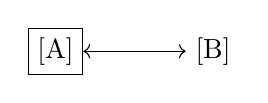
\begin{tikzpicture}
                \node[draw] (a) at (-1,0) {[A]}; \node (b) at (1,0) {[B]}; \draw[<->] (a) -- (b);
            \end{tikzpicture}
        \end{center}
        
        % Listing of code for the second example figure
        \item<+-> \texttt{\textbackslash node[draw,shape=circle,rotate=90] at (-1,0) \{\$1\$\}; \textbackslash node[draw=blue,very thick,shape=circle,fill=red,opacity=0.5,anchor=south] (b) at (1,0) \{\$2\$\}; \textbackslash draw[-latex,thick,dashdotted] (a.south) --++ (0,-0.4) --++ (1,0) -- (b.west) node[midway,above,rotate=60] \{middle\};}
        % Second example. MODIFY HERE and EXPERIMENT.
        \begin{center}
            \begin{tikzpicture}
                \node[draw,shape=circle,rotate=90] at (-1,0) {$1$}; \node[draw=blue,very thick,shape=circle,fill=red,opacity=0.5,anchor=south] (b) at (1,0) {$2$}; \draw[-latex,thick,dashdotted] (a.south) --++ (0,-0.4) --++  (1,0) -- (b.west) node[midway,above,rotate=60] {middle};
            \end{tikzpicture}
        \end{center}
        
    \end{itemize}
    % Now, try to understand how the diagram in the previous slide, "Simply TikZ - ex." and experiment with it. What would you have done differently? 
\end{frame}

\begin{frame}{Simply TikZ + 3D + loops - ex.}
    
    \vspace{-15pt}

    \begin{center}
        % Thanks to the array package, it is easy to create cells in a tabular with paragraph structure (text folding at the end of line, etc.). You need to specify the width, however.
        \begin{tabular}{m{.5\textwidth}m{.4\textwidth}}
            % The practical way of handling TikZ figures, as separate .tex files you input
            % Mathematical macros needed (related to paper content)
\newcommand{\supp}[1]{\operatorname{supp}\left( #1 \right)}
\def\sigmax{\sigma_{\max}}
\def\dsigma{\tilde{\sigma}}
\renewcommand{\complement}[1]{#1^{\mathsf{c}}}

% Define scaling variable
\def\sca{0.73}
% Set perspective for 3D rendering
\tdplotsetmaincoords{70}{110}

\begin{tikzpicture}[tdplot_main_coords,scale=\sca]
	% Define variables for drawing 
    	% Margin distance in x and min and max for sigma
		    \def\xdist{3.5} \def\sigminn{0} \def\sigmaxn{4.5}
	    % Margin distance in sigma and min and max for spatial coordinates
		    \def\sigdist{-2} \def\xmin{-.5} \def\xmax{-6} \def\ymin{0.25} \def\ymax{3.5}
		    
	% Draw support of spatial masking function 
		% Limits of spatial coordinates
		    \draw[blue] plot coordinates {(\xmin,\sigdist,\ymin) (\xmax,\sigdist,\ymin) (\xmax,\sigdist,\ymax) (\xmin,\sigdist,\ymax) (\xmin,\sigdist,\ymin)};
		    \node[color=blue] at (\xmax,\sigdist-1,\ymax+.2) {$\supp{\mu}$};
		% Guiding lines (observe \foreach)
		    \foreach \x in {\xmin,\xmax} {
			    \foreach \y in {\ymin,\ymax}{
				    \draw[thin,dashed,blue] (\x,\sigdist,\y) -- (\x,0,\y);
			    }
		    }
		
	% Grid for discretization of the spatial component
		% Configure variables
		    \def\nbins{5} \def\binsextra{2}
		% Set PGF variables as mathematical expressions of other variables
		    \pgfmathsetmacro{\nbinsextrapo}{-\binsextra +1} \pgfmathsetmacro{\nbinsextra}{\nbins +\binsextra}
		    \pgfmathsetmacro{\xbynbins}{(\xmax-\xmin)/\nbins} \pgfmathsetmacro{\ybynbins}{(\ymax-\ymin)/\nbins}
		% Draw spatial grid
		% Observe \foreach extrapolation \n in {0, 1, ..., 5}
		    \foreach \n in {-\binsextra, \nbinsextrapo, ...,\nbinsextra}{
			    % X divisions
			        \draw[gray!40,thin] (\xmin + \n*\xbynbins,0,\ymin-\binsextra*\ybynbins) -- (\xmin + \n*\xbynbins,0,\ymin+\nbinsextra*\ybynbins);
			    % Y divisions
			        \draw[gray!40,thin] (\xmin-\binsextra*\xbynbins,0,\ymin + \n*\ybynbins) -- (\xmin+\nbinsextra*\xbynbins,0,\ymin + \n*\ybynbins);
		    }
		% Draw box around spatial grid
		    \draw[thin] (\xmin -\binsextra*\xbynbins,0,\ymin-\binsextra*\ybynbins) -- (\xmin+\nbinsextra*\xbynbins,0,\ymin-\binsextra*\ybynbins) -- (\xmin+\nbinsextra*\xbynbins,0,\ymin+\nbinsextra*\ybynbins) node[anchor=south] {\textcolor{gray}{sensor's grid}} --	(\xmin-\binsextra*\xbynbins,0,\ymin+\nbinsextra*\ybynbins) -- cycle;
		% Draw mask support on the same level as the sensor grid
		\draw[blue,thin,dashed] plot coordinates {(\xmin,0,\ymin) (\xmax,0,\ymin) (\xmax,0,\ymax) (\xmin,0,\ymax) (\xmin,0,\ymin)};
		
	% Draw sigma discretization grid
		% Limits of sigma regions (note path does not end until ;)
		    \draw[red] (.1+\xdist,0,0) -- (-.1+\xdist,0,0) -- % Beginning tick
			(\xdist,\sigminn,0)  -- node[midway,below]{$\left[0,\sigmax\right]$} (\xdist,\sigmaxn,0) -- % Margins
			(.1+\xdist,\sigmaxn,0) -- (-.1+\xdist,\sigmaxn,0); % Ending tick
		% Guiding lines
		    \draw[thin,dashed,red] (\xdist,0,0) -- (0,0,0);
		    \draw[thin,dashed,red] (\xdist,4.5,0) -- (0,4.5,0);
		% Line for marking discretization of sigma
		    \draw[gray,thin] (.25*\xdist,\sigminn,0) -- (.25*\xdist,\sigmaxn,0);
		% Set PGF variable to length of sigma 
 		    \pgfmathsetmacro{\lofsig}{\sigmaxn-\sigminn}
 		% Mark discretization of sigma in line
 		    \foreach \prop in {0, .15, .25, .333, .5, .75, 1}{
			    \draw (.1+.25*\xdist,\prop*\lofsig,0) -- (-.1+.25*\xdist,\prop*\lofsig,0);
 			}
 		% Mark set of sigmas aleph and its complement
     		\draw[red,thin] (.5*\xdist,\sigminn,0) -- node[midway,below]{\scriptsize $\aleph$} (.5*\xdist,\sigminn+.75*\lofsig,0);
     		\draw[red,thin] (.5*\xdist,\sigminn+.75*\lofsig,0) -- node[midway,below]{\scriptsize $\complement{\aleph}$} (.5*\xdist,\sigmaxn,0);
 		% Guiding lines for aleph and its complement
     		\foreach \prop in {0, .75, 1}{
    			% Divisions in sigma axis
     			\draw[red,thin] (.1+.5*\xdist,\prop*\lofsig,0) -- (-.1+.5*\xdist,\prop*\lofsig,0);
     			% Divisions in 2D Space
     			\draw[red,thin,dashed] (.5*\xdist,\prop*\lofsig,0) -- (0,\prop*\lofsig,0);
     		}
	
	% Draw discrete axis (m,n,k)
	    % Spatial axis (m,n)
	        \draw[thick,->] (\xmin-\binsextra*\xbynbins,0,\ymin-\binsextra*\ybynbins) -- (\xmin-\binsextra*\xbynbins+.5*\xbynbins,0,\ymin-\binsextra*\ybynbins) node[anchor=west]{\tiny $\mathbf{n}$};
	        \draw[thick,->] (\xmin-\binsextra*\xbynbins,0,\ymin-\binsextra*\ybynbins) -- (\xmin-\binsextra*\xbynbins,0,\ymin+.5*\ybynbins-\binsextra*\ybynbins) node[anchor=east]{\tiny $\mathbf{m}$};
	    % Third dimension k
	        \draw[thick,->] (.25*\xdist,0,0) -- (.25*\xdist,.08*\lofsig,0) node[anchor=north east]{\tiny $\mathbf{k}$};
	
	% Draw example discretization regions
	    % Set parameters for the region to draw
	    \def\m{2} \def\n{1} \def\sigselmin{.15} \def\sigselmax{.25} 
	    % Call external (parametrized) tikz code
    	% Thought for use inside discretization_grid.tex only. Takes ``arguments'' from defined macros and
% plots the corresponding discretization region.	
	
	% Set PGF variables as mathematical expressions of other variables
	    \pgfmathsetmacro{\mpo}{\m+1} \pgfmathsetmacro{\npo}{\n+1}
	% Draw square on xy plane
	    \draw[dashed] (\xmin+\n*\xbynbins,0,\ymin+\m*\ybynbins) -- (\xmin+\npo*\xbynbins,0,\ymin+\m*\ybynbins) --
			(\xmin+\npo*\xbynbins,0,\ymin+\mpo*\ybynbins) -- (\xmin+\n*\xbynbins,0,\ymin+\mpo*\ybynbins) --
			(\xmin+\n*\xbynbins,0,\ymin+\m*\ybynbins);
	% Throw lines from the corners of the selected xy square
	    \draw[thin,dashed,gray!60] (\xmin+\n*\xbynbins,0,\ymin+\m*\ybynbins) -- (\xmin+\n*\xbynbins,\sigmaxn,\ymin+\m*\ybynbins);
	    \draw[thin,dashed,gray!60] (\xmin+\npo*\xbynbins,0,\ymin+\m*\ybynbins) -- (\xmin+\npo*\xbynbins,\sigmaxn,\ymin+\m*\ybynbins);
	    \draw[thin,dashed,gray!60] (\xmin+\npo*\xbynbins,0,\ymin+\mpo*\ybynbins) -- (\xmin+\npo*\xbynbins,\sigmaxn,\ymin+\mpo*\ybynbins);
	    \draw[thin,dashed,gray!60] (\xmin+\n*\xbynbins,0,\ymin+\mpo*\ybynbins) -- (\xmin+\n*\xbynbins,\sigmaxn,\ymin+\mpo*\ybynbins);
	% Draw selected segment on \sigma dimension
	    \draw[dashed] (.25*\xdist,\sigselmin*\lofsig,0) -- (.25*\xdist,\sigselmax*\lofsig,0);
	% Throw lines from the corners of the selected segment
	    \draw[thin,dashed,gray!60] (.25*\xdist,\sigselmin*\lofsig,0) -- (\xmax,\sigselmin*\lofsig,0);
	    \draw[thin,dashed,gray!60] (.25*\xdist,\sigselmax*\lofsig,0) -- (\xmax,\sigselmax*\lofsig,0);
	% Draw selected segment on \sigma-x plane
	    \draw[dashed] (\xmin+\n*\xbynbins,\sigselmin*\lofsig,0) -- (\xmin+\npo*\xbynbins,\sigselmin*\lofsig,0) -- (\xmin+\npo*\xbynbins,\sigselmax*\lofsig,0) -- (\xmin+\n*\xbynbins,\sigselmax*\lofsig,0) -- (\xmin+\n*\xbynbins,\sigselmin*\lofsig,0);
	% Throw lines upwards from the corners of the selected \sigma-x square
	    \draw[thin,dashed,gray!60] (\xmin+\n*\xbynbins,\sigselmin*\lofsig,0) -- (\xmin+\n*\xbynbins,\sigselmin*\lofsig,\ymax);
	    \draw[thin,dashed,gray!60] (\xmin+\npo*\xbynbins,\sigselmin*\lofsig,0) -- (\xmin+\npo*\xbynbins,\sigselmin*\lofsig,\ymax);
	    \draw[thin,dashed,gray!60] (\xmin+\npo*\xbynbins,\sigselmax*\lofsig,0) -- (\xmin+\npo*\xbynbins,\sigselmax*\lofsig,\ymax);
	    \draw[thin,dashed,gray!60] (\xmin+\n*\xbynbins,\sigselmax*\lofsig,0) -- (\xmin+\n*\xbynbins,\sigselmax*\lofsig,\ymax);
	% Highlight selected discretization region	
		% Foreground cube layer
		    \draw[thick] (\xmin+\n*\xbynbins,\sigselmin*\lofsig,\ymin+\m*\ybynbins) -- (\xmin+\n*\xbynbins,\sigselmin*\lofsig,\ymin+\mpo*\ybynbins) -- (\xmin+\n*\xbynbins,\sigselmax*\lofsig,\ymin+\mpo*\ybynbins) -- (\xmin+\n*\xbynbins,\sigselmax*\lofsig,\ymin+\m*\ybynbins) -- cycle;
		% Unseen cube lines
		    \draw[thick,dashed] (\xmin+\n*\xbynbins,\sigselmin*\lofsig,\ymin+\m*\ybynbins) -- (\xmin+\npo*\xbynbins,\sigselmin*\lofsig,\ymin+\m*\ybynbins) -- (\xmin+\npo*\xbynbins,\sigselmax*\lofsig,\ymin+\m*\ybynbins);
		    \draw[thick,dashed] (\xmin+\npo*\xbynbins,\sigselmin*\lofsig,\ymin+\m*\ybynbins) -- (\xmin+\npo*\xbynbins,\sigselmin*\lofsig,\ymin+\mpo*\ybynbins);
		% Lid cube layer
		    \draw[thick] (\xmin+\n*\xbynbins,\sigselmin*\lofsig,\ymin+\mpo*\ybynbins) -- (\xmin+\npo*\xbynbins,\sigselmin*\lofsig,\ymin+\mpo*\ybynbins) -- (\xmin+\npo*\xbynbins,\sigselmax*\lofsig,\ymin+\mpo*\ybynbins) -- (\xmin+\n*\xbynbins,\sigselmax*\lofsig,\ymin+\mpo*\ybynbins) -- cycle;
		% Remaining cube lines
		\draw[thick] (\xmin+\npo*\xbynbins,\sigselmax*\lofsig,\ymin+\mpo*\ybynbins) -- (\xmin+\npo*\xbynbins,\sigselmax*\lofsig,\ymin+\m*\ybynbins) --	(\xmin+\n*\xbynbins,\sigselmax*\lofsig,\ymin+\m*\ybynbins);
	    % Set parameters for the region to draw
	    \def\m{4} \def\n{4} \def\sigselmin{.75} \def\sigselmax{1} 
	    % Call external (parametrized) tikz code
	    % Thought for use inside discretization_grid.tex only. Takes ``arguments'' from defined macros and
% plots the corresponding discretization region.	
	
	% Set PGF variables as mathematical expressions of other variables
	    \pgfmathsetmacro{\mpo}{\m+1} \pgfmathsetmacro{\npo}{\n+1}
	% Draw square on xy plane
	    \draw[dashed] (\xmin+\n*\xbynbins,0,\ymin+\m*\ybynbins) -- (\xmin+\npo*\xbynbins,0,\ymin+\m*\ybynbins) --
			(\xmin+\npo*\xbynbins,0,\ymin+\mpo*\ybynbins) -- (\xmin+\n*\xbynbins,0,\ymin+\mpo*\ybynbins) --
			(\xmin+\n*\xbynbins,0,\ymin+\m*\ybynbins);
	% Throw lines from the corners of the selected xy square
	    \draw[thin,dashed,gray!60] (\xmin+\n*\xbynbins,0,\ymin+\m*\ybynbins) -- (\xmin+\n*\xbynbins,\sigmaxn,\ymin+\m*\ybynbins);
	    \draw[thin,dashed,gray!60] (\xmin+\npo*\xbynbins,0,\ymin+\m*\ybynbins) -- (\xmin+\npo*\xbynbins,\sigmaxn,\ymin+\m*\ybynbins);
	    \draw[thin,dashed,gray!60] (\xmin+\npo*\xbynbins,0,\ymin+\mpo*\ybynbins) -- (\xmin+\npo*\xbynbins,\sigmaxn,\ymin+\mpo*\ybynbins);
	    \draw[thin,dashed,gray!60] (\xmin+\n*\xbynbins,0,\ymin+\mpo*\ybynbins) -- (\xmin+\n*\xbynbins,\sigmaxn,\ymin+\mpo*\ybynbins);
	% Draw selected segment on \sigma dimension
	    \draw[dashed] (.25*\xdist,\sigselmin*\lofsig,0) -- (.25*\xdist,\sigselmax*\lofsig,0);
	% Throw lines from the corners of the selected segment
	    \draw[thin,dashed,gray!60] (.25*\xdist,\sigselmin*\lofsig,0) -- (\xmax,\sigselmin*\lofsig,0);
	    \draw[thin,dashed,gray!60] (.25*\xdist,\sigselmax*\lofsig,0) -- (\xmax,\sigselmax*\lofsig,0);
	% Draw selected segment on \sigma-x plane
	    \draw[dashed] (\xmin+\n*\xbynbins,\sigselmin*\lofsig,0) -- (\xmin+\npo*\xbynbins,\sigselmin*\lofsig,0) -- (\xmin+\npo*\xbynbins,\sigselmax*\lofsig,0) -- (\xmin+\n*\xbynbins,\sigselmax*\lofsig,0) -- (\xmin+\n*\xbynbins,\sigselmin*\lofsig,0);
	% Throw lines upwards from the corners of the selected \sigma-x square
	    \draw[thin,dashed,gray!60] (\xmin+\n*\xbynbins,\sigselmin*\lofsig,0) -- (\xmin+\n*\xbynbins,\sigselmin*\lofsig,\ymax);
	    \draw[thin,dashed,gray!60] (\xmin+\npo*\xbynbins,\sigselmin*\lofsig,0) -- (\xmin+\npo*\xbynbins,\sigselmin*\lofsig,\ymax);
	    \draw[thin,dashed,gray!60] (\xmin+\npo*\xbynbins,\sigselmax*\lofsig,0) -- (\xmin+\npo*\xbynbins,\sigselmax*\lofsig,\ymax);
	    \draw[thin,dashed,gray!60] (\xmin+\n*\xbynbins,\sigselmax*\lofsig,0) -- (\xmin+\n*\xbynbins,\sigselmax*\lofsig,\ymax);
	% Highlight selected discretization region	
		% Foreground cube layer
		    \draw[thick] (\xmin+\n*\xbynbins,\sigselmin*\lofsig,\ymin+\m*\ybynbins) -- (\xmin+\n*\xbynbins,\sigselmin*\lofsig,\ymin+\mpo*\ybynbins) -- (\xmin+\n*\xbynbins,\sigselmax*\lofsig,\ymin+\mpo*\ybynbins) -- (\xmin+\n*\xbynbins,\sigselmax*\lofsig,\ymin+\m*\ybynbins) -- cycle;
		% Unseen cube lines
		    \draw[thick,dashed] (\xmin+\n*\xbynbins,\sigselmin*\lofsig,\ymin+\m*\ybynbins) -- (\xmin+\npo*\xbynbins,\sigselmin*\lofsig,\ymin+\m*\ybynbins) -- (\xmin+\npo*\xbynbins,\sigselmax*\lofsig,\ymin+\m*\ybynbins);
		    \draw[thick,dashed] (\xmin+\npo*\xbynbins,\sigselmin*\lofsig,\ymin+\m*\ybynbins) -- (\xmin+\npo*\xbynbins,\sigselmin*\lofsig,\ymin+\mpo*\ybynbins);
		% Lid cube layer
		    \draw[thick] (\xmin+\n*\xbynbins,\sigselmin*\lofsig,\ymin+\mpo*\ybynbins) -- (\xmin+\npo*\xbynbins,\sigselmin*\lofsig,\ymin+\mpo*\ybynbins) -- (\xmin+\npo*\xbynbins,\sigselmax*\lofsig,\ymin+\mpo*\ybynbins) -- (\xmin+\n*\xbynbins,\sigselmax*\lofsig,\ymin+\mpo*\ybynbins) -- cycle;
		% Remaining cube lines
		\draw[thick] (\xmin+\npo*\xbynbins,\sigselmax*\lofsig,\ymin+\mpo*\ybynbins) -- (\xmin+\npo*\xbynbins,\sigselmax*\lofsig,\ymin+\m*\ybynbins) --	(\xmin+\n*\xbynbins,\sigselmax*\lofsig,\ymin+\m*\ybynbins);
	
	% Draw coordinate axis (x,\sigma,y)
	    \draw[thick,->] (0,0,0) -- (-9,0,0) node[anchor=north west]{$x$};
	    \draw[thick,->] (0,0,0) -- (0,5,0) node[anchor=south east]{$\dsigma$};
	    \draw[thick,->] (0,0,0) -- (0,0,5) node[anchor=south]{$y$};
\end{tikzpicture}
            % Explore the use of variables (\def), commands (\newcommand), for loops (\foreach) and color definitions (gray!40 = gray!40!white) in the published figure in figs/discretization_grid. MODIFY and EXPERIMENT. The simplicity of 3D comes from the great package tikz-3dplot.
            &
            % Listing of new concepts with respect to the previous
            \begin{itemize}
                \item More concepts and keywords: \texttt{\textbackslash def}, \texttt{\textbackslash foreach}, \texttt{\textbackslash pgfmathsetmacro}, \texttt{gray!40!blue}, \texttt{\textbackslash newcommand}
            \end{itemize}
            % Citation to paper where this figure appears
            {\footnotesize 
                Part of \fullcite{AguilaPla2017}
            }
        \end{tabular}
    \end{center}
\end{frame}

\begin{frame}{Simply TikZ for plotting}

    \vspace{-10pt}
    
    \begin{center}
        % Explore the use of 'plot file', 'plot function', and the keywords 'domain' and 'samples'. MODIFY and EXPERIMENT.
        
        % Set the scales of each axis and start figure
        \begin{tikzpicture}[xscale=1,yscale=15]
            % Draw axis
                \draw [->] (0,0) -- (0,0.3) node [anchor=south] {$f_x(x)$};
                \draw [->] (-5,0) -- (5.1,0) node [anchor=west] {$x$};
            % Draw labels
            % X axis
                \foreach \x in {-5, -4, ..., 5}
                    \draw (\x,0) node[anchor=north] {\scriptsize $\x$};
            % Y axis (with arbitrary labels, double for)
                \foreach \y/\ytext in {0.125/\tfrac{1}{8},0.25/\tfrac{1}{4}}
                    \draw (0,\y) node[anchor=west] {\scriptsize $\ytext$};
            
            % Plot for the actual distribution of some data
            % EXPERIMENT with changing the function expression
            % what happens with less samples?
                \draw[smooth,domain=-5:5,samples=400] plot 
                function{ (1/sqrt(2*pi))*( % Gaussian normalization factor (with std = 1)
                0.5*sqrt(2)*exp((-(x+2)**2))+ % Gaussian with weight (prob) 0.25 and stdeviation 1/sqrt(2) around -2
                0.5*exp((-(x-1)**2)/2))}; % Gaussain with weight (prob) 0.75 and stdeviation 1 around 1
            
            % Plot sampled data
                % The file data.txt is only two columns of numbers separated by spaces, check it out.
                \draw plot[only marks, mark=*, mark size=0.07pt, mark options={color=red!80}] file{figs/data.txt};
                
            % Plot histogram estimation
                % Why set the fill opacity at 0.5? Does it help for this figure?
                \draw[fill=orange, fill opacity=0.5] plot[ybar] file{figs/hist.txt};
                \draw[orange] node at (4,0.27) {\scriptsize Histogram};
            
            % Plot parametric model fittings
                % What does smooth do? let's try to change the colors, thicknesses, opacities, etc? What if we want markers to indicate the data points?
                \draw[color=blue] plot[smooth] file{figs/gen_pareto.txt};
                \draw[color=red] plot[smooth] file{figs/gen_extr_value.txt};
                \draw[color=green] plot [smooth] file{figs/normal.txt};
            
            % Names of parametric model fittings (note the equivalence between \node and \draw node
                \node at (4,0.30) {\scriptsize True distribution};
                \draw[color=blue] node at (4,0.24) {\scriptsize Generalized Pareto};
                \draw[color=red] node at (4,0.21) {\scriptsize Generalized Extreme Value};
                \draw[color=green] node at (4,0.18) {\scriptsize Normal};
            
      \end{tikzpicture}
      \end{center}
      
      \vspace{-20pt}
      
      \begin{itemize}
          \item More concepts and keywords: \texttt{plot file}, \texttt{smooth}, \texttt{ybar}, \texttt{plot function}, \texttt{domain}, \texttt{samples}
      \end{itemize}
      
      \small Part of an old presentation - will not be published.
      
\end{frame}

\begin{frame}{Simply TikZ scripted plotting - ex.}
    
    \vspace{-15pt}
    
    \begin{center}
        % See file, mainly generated by a MATLAB script that writes out TikZ lines after computing the statistics of the results. Extremely easy to script using fprintf onto an open file.
        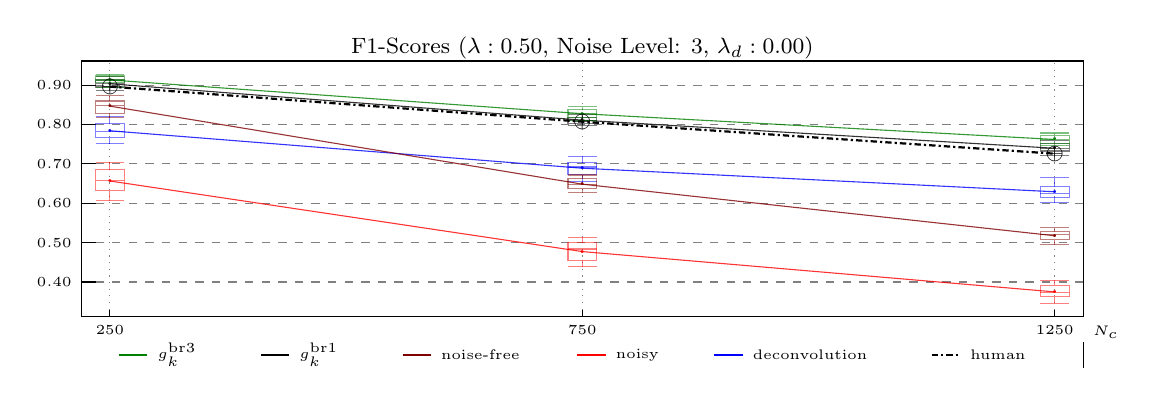
\begin{tikzpicture}[xscale=0.12,yscale=5]
	\def\ww{1.515152}\def\bw{1.515152}\def\xm{1.515152}\def\ym{0.016622}
	\fill[white] (25.000000-2*\xm,0.346073-2*\ym) rectangle (125.000000+2*\xm,0.927834+2*\ym);
	\draw (25.000000-2*\xm,0.346073-2*\ym) -- (125.000000+2*\xm,0.346073-2*\ym) -- (125.000000+2*\xm,0.927834+2*\ym) -- (25.000000-2*\xm,0.927834+2*\ym) -- cycle;
\node at (125.000000+2*\xm,0.346073-2*\ym) [anchor=north west]{\tiny $N_c$};

	\foreach \x/\n in {25/250,75/750,125/1250}{ \draw (\x,0.346073-\ym) -- (\x,0.346073-2*\ym) node[anchor=north,rotate=0]{\tiny $\n$}; \draw[thin,dotted,gray] (\x,0.346073-\ym) -- (\x,0.927834+2*\ym); }
	\foreach \y in {0.40,0.50,0.60,0.70,0.80,0.90}{ \draw (25.000000-\xm,\y) -- (25.000000-2*\xm,\y) node[anchor=east]{\tiny $\y$};  \draw[thin,dashed,gray] (25.000000-\xm,\y) -- (125.000000+2*\xm,\y); }
\node at (75.000000,0.927834+4*\ym) {\footnotesize F1-Scores ($\lambda: 0.50$, Noise Level: $ 3$, $\lambda_d: 0.00$)};

	%              
		\draw[black,opacity = 0.5] (25.000000-\ww,0.886597) -- (25.000000+\ww,0.886597);\draw[black,opacity = 0.5] (25.000000-\ww,0.920829) -- (25.000000+\ww,0.920829);
\draw[black,opacity = 0.5] (25.000000,0.886597) -- (25.000000,0.895075);\draw[black,opacity = 0.5] (25.000000,0.912863) -- (25.000000,0.920829);		\draw[black,opacity = 0.5] (25.000000-\bw,0.895075) -- (25.000000+\bw,0.895075) -- (25.000000+\bw,0.912863) -- (25.000000-\bw,0.912863) -- cycle;
		\draw[black,opacity = 0.5] (25.000000-\bw,0.903766) -- (25.000000+\bw,0.903766);
		\node[color=black] at (25.000000,0.903380) {.};
		\draw[black,opacity = 0.5] (75.000000-\ww,0.798175) -- (75.000000+\ww,0.798175);\draw[black,opacity = 0.5] (75.000000-\ww,0.826384) -- (75.000000+\ww,0.826384);
\draw[black,opacity = 0.5] (75.000000,0.798175) -- (75.000000,0.803371);\draw[black,opacity = 0.5] (75.000000,0.817159) -- (75.000000,0.826384);		\draw[black,opacity = 0.5] (75.000000-\bw,0.803371) -- (75.000000+\bw,0.803371) -- (75.000000+\bw,0.817159) -- (75.000000-\bw,0.817159) -- cycle;
		\draw[black,opacity = 0.5] (75.000000-\bw,0.809255) -- (75.000000+\bw,0.809255);
		\node[color=black] at (75.000000,0.810948) {.};
		\draw[black,opacity = 0.5] (125.000000-\ww,0.720190) -- (125.000000+\ww,0.720190);\draw[black,opacity = 0.5] (125.000000-\ww,0.758380) -- (125.000000+\ww,0.758380);
\draw[black,opacity = 0.5] (125.000000,0.720190) -- (125.000000,0.732648);\draw[black,opacity = 0.5] (125.000000,0.752475) -- (125.000000,0.758380);		\draw[black,opacity = 0.5] (125.000000-\bw,0.732648) -- (125.000000+\bw,0.732648) -- (125.000000+\bw,0.752475) -- (125.000000-\bw,0.752475) -- cycle;
		\draw[black,opacity = 0.5] (125.000000-\bw,0.738859) -- (125.000000+\bw,0.738859);
		\node[color=black] at (125.000000,0.739516) {.};
		\draw[black,opacity=0.8] (25.000000,0.903380) -- (75.000000,0.810948) -- (125.000000,0.739516);

	%
		\draw[black!50!green,opacity = 0.5] (25.000000-\ww,0.894705) -- (25.000000+\ww,0.894705);\draw[black!50!green,opacity = 0.5] (25.000000-\ww,0.927834) -- (25.000000+\ww,0.927834);
\draw[black!50!green,opacity = 0.5] (25.000000,0.894705) -- (25.000000,0.906054);\draw[black!50!green,opacity = 0.5] (25.000000,0.923077) -- (25.000000,0.927834);		\draw[black!50!green,opacity = 0.5] (25.000000-\bw,0.906054) -- (25.000000+\bw,0.906054) -- (25.000000+\bw,0.923077) -- (25.000000-\bw,0.923077) -- cycle;
		\draw[black!50!green,opacity = 0.5] (25.000000-\bw,0.912821) -- (25.000000+\bw,0.912821);
		\node[color=black!50!green] at (25.000000,0.913165) {.};
		\draw[black!50!green,opacity = 0.5] (75.000000-\ww,0.811042) -- (75.000000+\ww,0.811042);\draw[black!50!green,opacity = 0.5] (75.000000-\ww,0.844806) -- (75.000000+\ww,0.844806);
\draw[black!50!green,opacity = 0.5] (75.000000,0.811042) -- (75.000000,0.817280);\draw[black!50!green,opacity = 0.5] (75.000000,0.837631) -- (75.000000,0.844806);		\draw[black!50!green,opacity = 0.5] (75.000000-\bw,0.817280) -- (75.000000+\bw,0.817280) -- (75.000000+\bw,0.837631) -- (75.000000-\bw,0.837631) -- cycle;
		\draw[black!50!green,opacity = 0.5] (75.000000-\bw,0.828628) -- (75.000000+\bw,0.828628);
		\node[color=black!50!green] at (75.000000,0.827332) {.};
		\draw[black!50!green,opacity = 0.5] (125.000000-\ww,0.746938) -- (125.000000+\ww,0.746938);\draw[black!50!green,opacity = 0.5] (125.000000-\ww,0.778296) -- (125.000000+\ww,0.778296);
\draw[black!50!green,opacity = 0.5] (125.000000,0.746938) -- (125.000000,0.752467);\draw[black!50!green,opacity = 0.5] (125.000000,0.771990) -- (125.000000,0.778296);		\draw[black!50!green,opacity = 0.5] (125.000000-\bw,0.752467) -- (125.000000+\bw,0.752467) -- (125.000000+\bw,0.771990) -- (125.000000-\bw,0.771990) -- cycle;
		\draw[black!50!green,opacity = 0.5] (125.000000-\bw,0.761166) -- (125.000000+\bw,0.761166);
		\node[color=black!50!green] at (125.000000,0.761891) {.};
		\draw[black!50!green,opacity=0.8] (25.000000,0.913165) -- (75.000000,0.827332) -- (125.000000,0.761891);

	%
		\draw[blue,opacity = 0.5] (25.000000-\ww,0.750868) -- (25.000000+\ww,0.750868);\draw[blue,opacity = 0.5] (25.000000-\ww,0.819761) -- (25.000000+\ww,0.819761);
\draw[blue,opacity = 0.5] (25.000000,0.750868) -- (25.000000,0.766440);\draw[blue,opacity = 0.5] (25.000000,0.802752) -- (25.000000,0.819761);		\draw[blue,opacity = 0.5] (25.000000-\bw,0.766440) -- (25.000000+\bw,0.766440) -- (25.000000+\bw,0.802752) -- (25.000000-\bw,0.802752) -- cycle;
		\draw[blue,opacity = 0.5] (25.000000-\bw,0.782393) -- (25.000000+\bw,0.782393);
		\node[color=blue] at (25.000000,0.783990) {.};
		\draw[blue,opacity = 0.5] (75.000000-\ww,0.654692) -- (75.000000+\ww,0.654692);\draw[blue,opacity = 0.5] (75.000000-\ww,0.717711) -- (75.000000+\ww,0.717711);
\draw[blue,opacity = 0.5] (75.000000,0.654692) -- (75.000000,0.672811);\draw[blue,opacity = 0.5] (75.000000,0.702362) -- (75.000000,0.717711);		\draw[blue,opacity = 0.5] (75.000000-\bw,0.672811) -- (75.000000+\bw,0.672811) -- (75.000000+\bw,0.702362) -- (75.000000-\bw,0.702362) -- cycle;
		\draw[blue,opacity = 0.5] (75.000000-\bw,0.691941) -- (75.000000+\bw,0.691941);
		\node[color=blue] at (75.000000,0.688855) {.};
		\draw[blue,opacity = 0.5] (125.000000-\ww,0.602345) -- (125.000000+\ww,0.602345);\draw[blue,opacity = 0.5] (125.000000-\ww,0.664335) -- (125.000000+\ww,0.664335);
\draw[blue,opacity = 0.5] (125.000000,0.602345) -- (125.000000,0.615093);\draw[blue,opacity = 0.5] (125.000000,0.642402) -- (125.000000,0.664335);		\draw[blue,opacity = 0.5] (125.000000-\bw,0.615093) -- (125.000000+\bw,0.615093) -- (125.000000+\bw,0.642402) -- (125.000000-\bw,0.642402) -- cycle;
		\draw[blue,opacity = 0.5] (125.000000-\bw,0.625698) -- (125.000000+\bw,0.625698);
		\node[color=blue] at (125.000000,0.629007) {.};
		\draw[blue,opacity=0.8] (25.000000,0.783990) -- (75.000000,0.688855) -- (125.000000,0.629007);

	%
		\draw[red,opacity = 0.5] (25.000000-\ww,0.606265) -- (25.000000+\ww,0.606265);\draw[red,opacity = 0.5] (25.000000-\ww,0.703765) -- (25.000000+\ww,0.703765);
\draw[red,opacity = 0.5] (25.000000,0.606265) -- (25.000000,0.631579);\draw[red,opacity = 0.5] (25.000000,0.684685) -- (25.000000,0.703765);		\draw[red,opacity = 0.5] (25.000000-\bw,0.631579) -- (25.000000+\bw,0.631579) -- (25.000000+\bw,0.684685) -- (25.000000-\bw,0.684685) -- cycle;
		\draw[red,opacity = 0.5] (25.000000-\bw,0.657626) -- (25.000000+\bw,0.657626);
		\node[color=red] at (25.000000,0.656423) {.};
		\draw[red,opacity = 0.5] (75.000000-\ww,0.438742) -- (75.000000+\ww,0.438742);\draw[red,opacity = 0.5] (75.000000-\ww,0.513283) -- (75.000000+\ww,0.513283);
\draw[red,opacity = 0.5] (75.000000,0.438742) -- (75.000000,0.455336);\draw[red,opacity = 0.5] (75.000000,0.499234) -- (75.000000,0.513283);		\draw[red,opacity = 0.5] (75.000000-\bw,0.455336) -- (75.000000+\bw,0.455336) -- (75.000000+\bw,0.499234) -- (75.000000-\bw,0.499234) -- cycle;
		\draw[red,opacity = 0.5] (75.000000-\bw,0.483674) -- (75.000000+\bw,0.483674);
		\node[color=red] at (75.000000,0.477120) {.};
		\draw[red,opacity = 0.5] (125.000000-\ww,0.346073) -- (125.000000+\ww,0.346073);\draw[red,opacity = 0.5] (125.000000-\ww,0.404413) -- (125.000000+\ww,0.404413);
\draw[red,opacity = 0.5] (125.000000,0.346073) -- (125.000000,0.363010);\draw[red,opacity = 0.5] (125.000000,0.391885) -- (125.000000,0.404413);		\draw[red,opacity = 0.5] (125.000000-\bw,0.363010) -- (125.000000+\bw,0.363010) -- (125.000000+\bw,0.391885) -- (125.000000-\bw,0.391885) -- cycle;
		\draw[red,opacity = 0.5] (125.000000-\bw,0.374256) -- (125.000000+\bw,0.374256);
		\node[color=red] at (125.000000,0.374687) {.};
		\draw[red,opacity=0.8] (25.000000,0.656423) -- (75.000000,0.477120) -- (125.000000,0.374687);

	%
		\draw[black!50!red,opacity = 0.5] (25.000000-\ww,0.817597) -- (25.000000+\ww,0.817597);\draw[black!50!red,opacity = 0.5] (25.000000-\ww,0.872611) -- (25.000000+\ww,0.872611);
\draw[black!50!red,opacity = 0.5] (25.000000,0.817597) -- (25.000000,0.828633);\draw[black!50!red,opacity = 0.5] (25.000000,0.859611) -- (25.000000,0.872611);		\draw[black!50!red,opacity = 0.5] (25.000000-\bw,0.828633) -- (25.000000+\bw,0.828633) -- (25.000000+\bw,0.859611) -- (25.000000-\bw,0.859611) -- cycle;
		\draw[black!50!red,opacity = 0.5] (25.000000-\bw,0.847060) -- (25.000000+\bw,0.847060);
		\node[color=black!50!red] at (25.000000,0.846573) {.};
		\draw[black!50!red,opacity = 0.5] (75.000000-\ww,0.627090) -- (75.000000+\ww,0.627090);\draw[black!50!red,opacity = 0.5] (75.000000-\ww,0.671644) -- (75.000000+\ww,0.671644);
\draw[black!50!red,opacity = 0.5] (75.000000,0.627090) -- (75.000000,0.636220);\draw[black!50!red,opacity = 0.5] (75.000000,0.662005) -- (75.000000,0.671644);		\draw[black!50!red,opacity = 0.5] (75.000000-\bw,0.636220) -- (75.000000+\bw,0.636220) -- (75.000000+\bw,0.662005) -- (75.000000-\bw,0.662005) -- cycle;
		\draw[black!50!red,opacity = 0.5] (75.000000-\bw,0.647570) -- (75.000000+\bw,0.647570);
		\node[color=black!50!red] at (75.000000,0.648362) {.};
		\draw[black!50!red,opacity = 0.5] (125.000000-\ww,0.494249) -- (125.000000+\ww,0.494249);\draw[black!50!red,opacity = 0.5] (125.000000-\ww,0.537271) -- (125.000000+\ww,0.537271);
\draw[black!50!red,opacity = 0.5] (125.000000,0.494249) -- (125.000000,0.507028);\draw[black!50!red,opacity = 0.5] (125.000000,0.527264) -- (125.000000,0.537271);		\draw[black!50!red,opacity = 0.5] (125.000000-\bw,0.507028) -- (125.000000+\bw,0.507028) -- (125.000000+\bw,0.527264) -- (125.000000-\bw,0.527264) -- cycle;
		\draw[black!50!red,opacity = 0.5] (125.000000-\bw,0.521102) -- (125.000000+\bw,0.521102);
		\node[color=black!50!red] at (125.000000,0.517301) {.};
		\draw[black!50!red,opacity=0.8] (25.000000,0.846573) -- (75.000000,0.648362) -- (125.000000,0.517301);
		
		\draw[black,thick,dash pattern=on 2.3pt off 1.1pt on 0.8pt off 1.1pt] (25,0.896247) node {\footnotesize $\oplus$} -- (75,0.806990) node {\footnotesize $\oplus$} -- (125,0.725790) node {\footnotesize $\oplus$};

        % Set variables for legend (scale and placement)
		\def\xmax{125+2*\xm} 
		\def\xmin{25-2*\xm}
		\def\ymax{0.346073-6*\ym}
		\def\legh{0.4/6.2}
		\def\indicatorw{0.3/0.1}
		% Draw rectangle and fill it up
\draw (\xmin,\ymax-\legh) rectangle (\xmax,\ymax);
\fill[white,fill opacity=1,opacity=1] (\xmin,\ymax-\legh) rectangle (\xmax,\ymax);
% Placement, name and colour for methods
\foreach \num/\name/\c in {0.04/$g_k^{\mathrm{br3}}$/black!50!green,
                           0.19/$g_k^{\mathrm{br1}}$/black,
                           0.34/noise-free/black!50!red,
                           0.525/noisy/red,
                           0.67/deconvolution/blue}{
    % Small line and name
    \draw[\c, thick] (\num*\xmax-\num*\xmin+\xmin,\ymax-\legh/2) -- (\num*\xmax-\num*\xmin+\xmin+\indicatorw,\ymax-\legh/2) node [anchor=west,color=black] {\tiny \name};
  }
% Placement, name and colour for human
\def\num{0.9} \def\name{human}
% Small line and name
\draw[black,dash pattern=on 2.3pt off 1.1pt on 0.8pt off 1.1pt,thick] (\num*\xmax-\num*\xmin+\xmin,\ymax-\legh/2) -- (\num*\xmax-\num*\xmin+\xmin+\indicatorw,\ymax-\legh/2) node [anchor=west,color=black] {\tiny \name};

\end{tikzpicture}

    \end{center}
    
    \vspace{-15pt}
    
    \begin{itemize}
        \item Easily scripted
    \end{itemize}
    {\footnotesize 
    Part of \fullcite{AguilaPla2017a}
    }
            
\end{frame}

\begin{frame}{PGFplots - Easier plotting}
    % Column environment from beamer. Good for this kind of alignment.
    \begin{columns}[T]
        % Figure column, EXPERIMENT here
        \begin{column}{.48\textwidth}
            % The simplicity of PGFplots is appealing. Try to configure this simple plot to your liking. Try adding markers. Can you set how many samples of the function are used for the drawing? Change the function, how does it behave compared to "Simply TikZ for plotting"? Can you set the minimum and maximum values for each axis?
            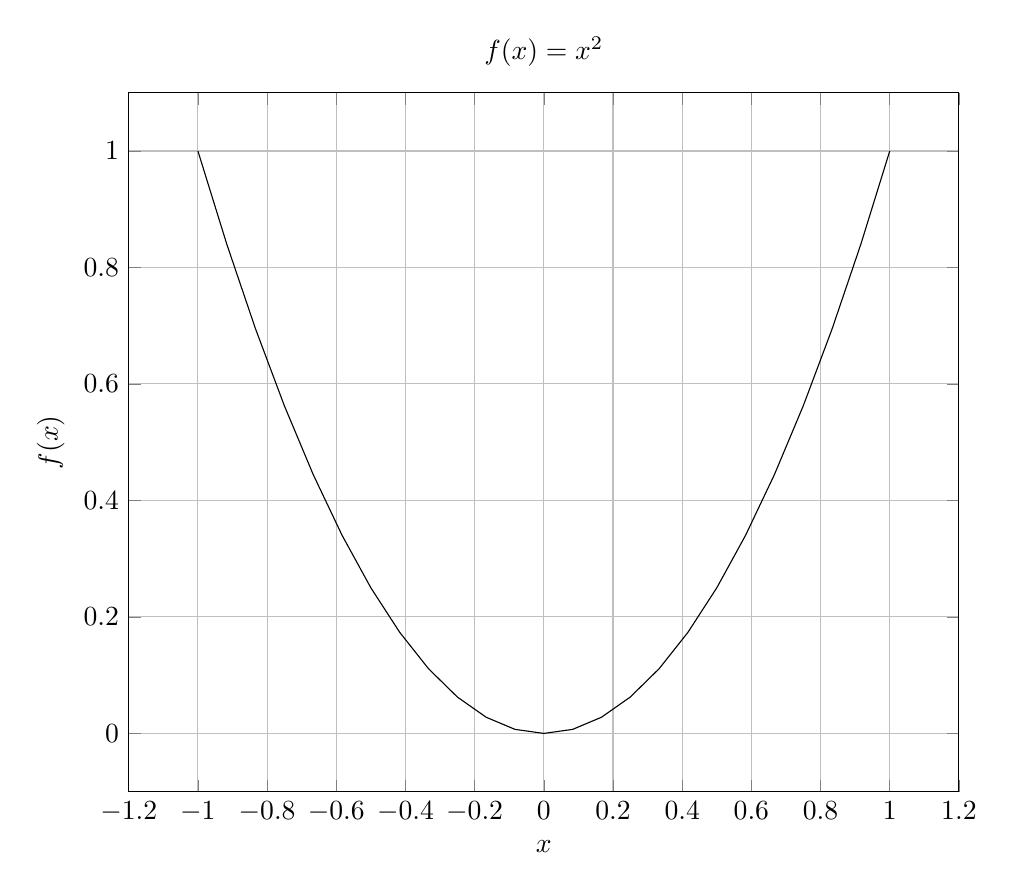
\begin{tikzpicture}
                \begin{axis}[
                    title = {$f(x) = x^2$},
                    grid = major,
                    xlabel = {$x$},
                    ylabel = {$f(x)$},
                    width=\textwidth
                ]
                    \addplot[domain = -1:1] {x^2};
                \end{axis}
            \end{tikzpicture}
        \end{column}\hfill
        % Listing of the code for the example figure
        \begin{column}{.48\textwidth}
            \vspace{40pt}
            \texttt{\textbackslash begin\{axis\}[
            title = \{\$f(x) = x\^{}2\$\},grid = major,xlabel = \{\$x\$\},ylabel = \{\$f(x)\$\},]
            \textbackslash addplot[domain = -1:1] \{x\^{}2\}; \textbackslash end\{axis\}}
        \end{column}
    \end{columns}
\end{frame}

\begin{frame}{PGFplots - Easier 3D plotting}
    \begin{columns}[T]
    % Figure column, EXPERIMENT here. Can you change the colours? Can you include a colorbar? Change the function and the number of samples.
    \begin{column}{.45\textwidth}
            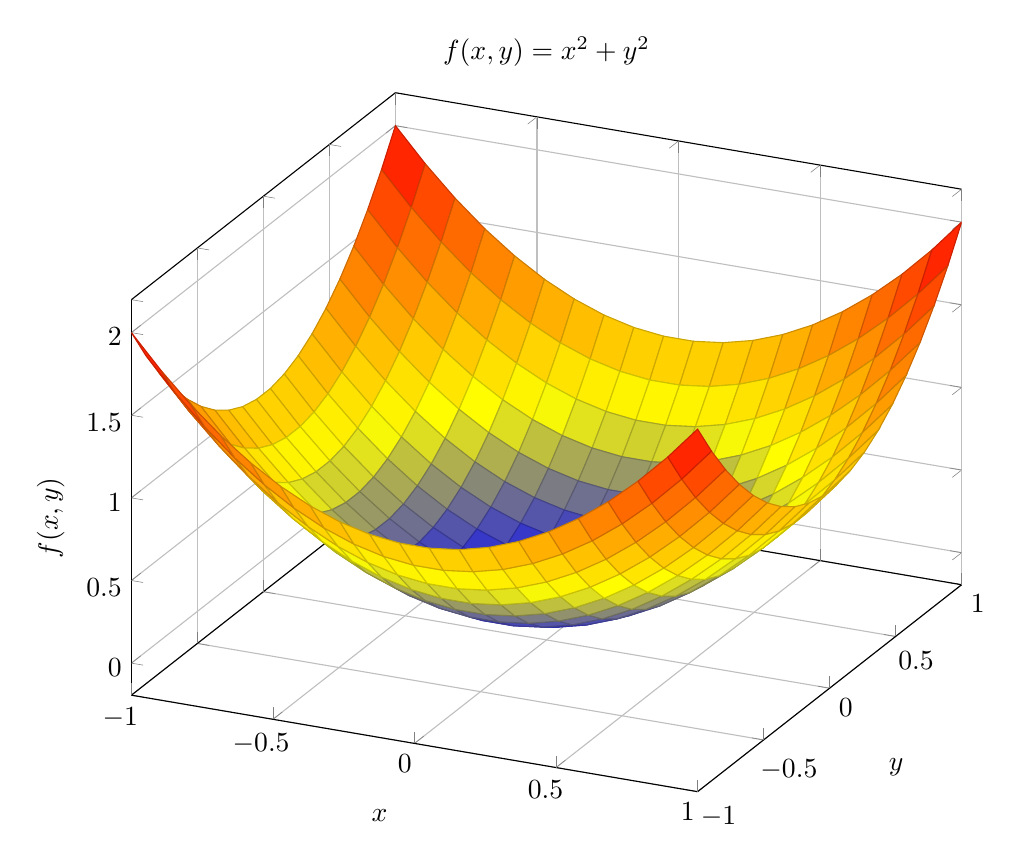
\begin{tikzpicture}
                \begin{axis}[title = {$f(x,y) = x^2 + y^2$},grid = major,xlabel = {$x$},ylabel = {$y$},zlabel={$f(x,y)$},width=\textwidth]
                    \addplot3[surf,domain = -1:1,samples=20] {x^2+y^2};
                \end{axis}
            \end{tikzpicture}
        \end{column}\hfill
        % Listing of the code for the example figure
        \begin{column}{.48\textwidth}
        
            \vspace{30pt}
        
            \texttt{\textbackslash begin\{axis\}[ title = \{ \$f(x,y) = x\^{}2 + y\^{}2\$\}, grid = major, xlabel = \{\$x\$\}, ylabel = \{\$y\$\},zlabel=\{\$f(x,y)\$\},]
                    \textbackslash addplot3[surf,domain = -1:1,samples=20] \{x\^{}2+y\^{}2\};
                \textbackslash end\{axis\}}
        \end{column}
    \end{columns}
\end{frame}

\begin{frame}{PGFplots from Python (matplotlib2tikz)}
    % If you are familiar with matplotlib, explore the screen capture of a Jupyter notebook on the slide
    \only<1>{
        \begin{center}
            \includegraphics[keepaspectratio=true,width=.95\textwidth]{figs/creating_example.png}
        \end{center}
    }
    % Simply importing the file saved by the Jupyter notebook, we obtain this very good starting point.
    \only<2>{
        \begin{columns}
            % Input figure
            \begin{column}{.58\textwidth}
                \input{figs/example}
            \end{column}\hfill
            % Listing of input figure
            \begin{column}{.4\textwidth}
                \texttt{\textbackslash input\{figs/example\} }
            \end{column}
        \end{columns}
    }
    % Small modifications provide an amazing-looking figure with scalable graphics, font integration, re-usability, and most of the other advantages of TikZ in minutes
    \only<3>{
        % EXPLORE the differences between 'figs/example' and 'figs/example_improved' and EXPERIMENT
        % This file was created by matplotlib2tikz v0.6.18 and then edited manually for best results
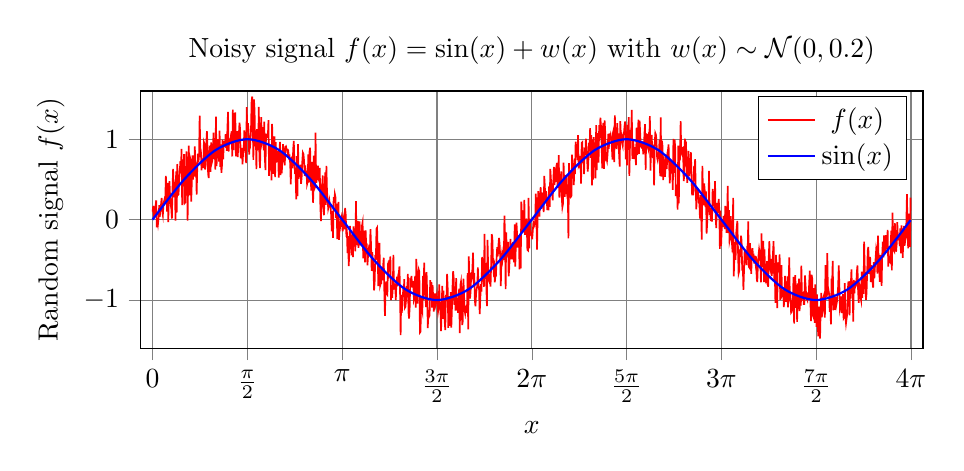
\begin{tikzpicture}
\begin{axis}[
width = .95\textwidth,
height = .4\textwidth,
tick align=outside,
tick pos=left,
title={Noisy signal $f(x) = \sin(x) + w(x)$ with $w(x)\sim\mathcal{N}(0,0.2)$},
x grid style={gray},
xlabel={$x$},
xmin=-0.2, xmax=12.766,
y grid style={gray},
ylabel={Random signal $f(x)$},
xtick =       {0,   1.57080,        3.14159, 4.71239,          6.28319, 7.85398, 9.42478, 10.99557,12.56637},
xticklabels = {$0$, $\frac{\pi}{2}$, $\pi$,  $\frac{3\pi}{2}$, $2\pi$, $\frac{5\pi}{2}$,$3\pi$,$\frac{7\pi}{2}$,$4\pi$},
ymin=-1.6, ymax=1.6,
grid = major,
]
\addplot [semithick, red]
table [row sep=\\]{%
0	0.0983183727617042 \\
0.01	0.169353489381384 \\
0.02	0.0241289382769289 \\
0.03	0.12235409835309 \\
0.04	0.0978070811132391 \\
0.05	0.174962862825925 \\
0.06	0.240150822545598 \\
0.07	-0.0964853840029278 \\
0.08	0.0162911683754095 \\
0.09	-0.0487626747674911 \\
0.1	0.023181374447477 \\
0.11	0.181030712918288 \\
0.12	0.0354310109985665 \\
0.13	0.159174158475916 \\
0.14	0.190680099138285 \\
0.15	0.269712083354608 \\
0.16	0.102989689388542 \\
0.17	0.0557311801692153 \\
0.18	0.184639003867061 \\
0.19	0.228083927065558 \\
0.2	0.26079373120713 \\
0.21	0.244385554821081 \\
0.22	0.54332827740805 \\
0.23	0.35458095336074 \\
0.24	0.0983960079209572 \\
0.25	0.456944085189749 \\
0.26	-0.0301973298308709 \\
0.27	0.341685778709847 \\
0.28	0.476836810649719 \\
0.29	0.277157441266594 \\
0.3	0.178792013640026 \\
0.31	0.138134286756507 \\
0.32	0.011577746508296 \\
0.33	0.39116647635873 \\
0.34	0.631835217690175 \\
0.35	0.276138437060142 \\
0.36	0.436928437444358 \\
0.37	0.393243601138354 \\
0.38	-0.0128333726379399 \\
0.39	0.59988439506831 \\
0.4	0.0888359608125257 \\
0.41	0.691554297604396 \\
0.42	0.306653237920584 \\
0.43	0.312569091130085 \\
0.44	0.480738042272105 \\
0.45	0.591845556918115 \\
0.46	0.726128256620511 \\
0.47	0.623872900257788 \\
0.48	0.880296094408114 \\
0.49	0.181598680388586 \\
0.5	0.745943837275046 \\
0.51	0.412787449827427 \\
0.52	0.814212231627482 \\
0.53	0.203368858288371 \\
0.54	0.212548862414811 \\
0.55	0.487255745007129 \\
0.56	0.849266796231216 \\
0.57	0.694859792021809 \\
0.58	-0.012705671840696 \\
0.59	0.544927107711436 \\
0.6	0.919320751326101 \\
0.61	0.301694153586442 \\
0.62	0.772800498563162 \\
0.63	0.740053533324033 \\
0.64	0.223409674266345 \\
0.65	0.463941892373548 \\
0.66	0.799122846392763 \\
0.67	0.49624553621 \\
0.68	0.797331013414131 \\
0.69	0.533680784424466 \\
0.7	0.91144947308418 \\
0.71	0.56511224532815 \\
0.72	0.707900113011665 \\
0.73	0.31056121503162 \\
0.74	0.638061021333477 \\
0.75	0.820944294673784 \\
0.76	0.713664254052961 \\
0.77	0.797366134592202 \\
0.78	1.29291323956066 \\
0.79	0.886846794484551 \\
0.8	0.861915690494494 \\
0.81	0.611816484348718 \\
0.82	0.742465764203826 \\
0.83	0.752532813202226 \\
0.84	0.640612750491653 \\
0.85	0.964719228664773 \\
0.86	0.942457660531747 \\
0.87	0.62217200405792 \\
0.88	0.678156812439513 \\
0.89	0.939215961300383 \\
0.9	1.09883080971781 \\
0.91	0.894708766717569 \\
0.92	0.572147907093172 \\
0.93	0.516474535818785 \\
0.94	0.81557848006077 \\
0.95	0.918997827527012 \\
0.96	0.59250529948157 \\
0.97	0.960191818789523 \\
0.98	0.703836401379806 \\
0.99	0.734584692073622 \\
1	0.883148350978519 \\
1.01	1.08198654262357 \\
1.02	0.752372011325778 \\
1.03	0.892833976482188 \\
1.04	0.623252082451168 \\
1.05	1.28142766718415 \\
1.06	0.666097772760832 \\
1.07	0.838391102335648 \\
1.08	1.00024307431139 \\
1.09	0.889003609866643 \\
1.1	0.723139295389075 \\
1.11	1.10739469441064 \\
1.12	0.655549827124643 \\
1.13	0.934488676843868 \\
1.14	0.581276791571777 \\
1.15	0.674230238872086 \\
1.16	0.994799851501107 \\
1.17	0.74882027227231 \\
1.18	0.975568338161601 \\
1.19	0.928959171922939 \\
1.2	0.918558642635972 \\
1.21	1.06412303919524 \\
1.22	0.944457889507615 \\
1.23	0.856236451625198 \\
1.24	1.14183763696165 \\
1.25	1.33855389442048 \\
1.26	0.844874712883071 \\
1.27	1.00672494354837 \\
1.28	0.94583204568795 \\
1.29	0.95474852433392 \\
1.3	1.05250908998728 \\
1.31	1.09750855517726 \\
1.32	0.785202638637096 \\
1.33	1.36904708644316 \\
1.34	0.865545359594296 \\
1.35	1.32490887485079 \\
1.36	0.960950715535009 \\
1.37	1.33362096873375 \\
1.38	0.786916439263991 \\
1.39	0.924890085763931 \\
1.4	1.10136416127193 \\
1.41	0.778472867216992 \\
1.42	0.915029436390285 \\
1.43	1.06436674165629 \\
1.44	1.20583773929427 \\
1.45	1.12494582104495 \\
1.46	0.762528356229245 \\
1.47	0.818557380237846 \\
1.48	0.892798316085053 \\
1.49	0.688485082698676 \\
1.5	0.823739077906203 \\
1.51	0.887358942746841 \\
1.52	1.11024755540072 \\
1.53	0.982726613867883 \\
1.54	0.8443006415469 \\
1.55	0.702228997856955 \\
1.56	1.39915612976381 \\
1.57	1.08747053495026 \\
1.58	1.19915908403867 \\
1.59	1.10840303837001 \\
1.6	0.808753824914862 \\
1.61	1.01921988227504 \\
1.62	0.970917887884871 \\
1.63	1.09857831831858 \\
1.64	1.45888788795374 \\
1.65	1.53045991646122 \\
1.66	1.18352926462618 \\
1.67	0.744382582506287 \\
1.68	1.49401862064452 \\
1.69	1.36036375192655 \\
1.7	0.912116786452003 \\
1.71	1.09033461729076 \\
1.72	0.628126962185344 \\
1.73	1.12431785842882 \\
1.74	1.04168799868282 \\
1.75	0.863438230165775 \\
1.76	1.40051973184019 \\
1.77	0.753807806360172 \\
1.78	0.640758786382268 \\
1.79	0.990630092843944 \\
1.8	1.27325724149412 \\
1.81	0.964115918965433 \\
1.82	1.00578840295713 \\
1.83	1.15089321066336 \\
1.84	0.862783991825811 \\
1.85	1.21782591508127 \\
1.86	0.770026363714041 \\
1.87	0.616150973085396 \\
1.88	1.06918634634018 \\
1.89	1.02267521991805 \\
1.9	1.02500338010898 \\
1.91	1.03613051365276 \\
1.92	1.23819129342431 \\
1.93	0.544835876111439 \\
1.94	0.933203837172366 \\
1.95	0.790229334554081 \\
1.96	0.922936561141119 \\
1.97	0.488223781158125 \\
1.98	1.19184919759973 \\
1.99	0.91606130264661 \\
2	0.567880941639687 \\
2.01	0.732972564048692 \\
2.02	1.0349803262669 \\
2.03	0.528243870003685 \\
2.04	0.964087313382733 \\
2.05	0.708781481216706 \\
2.06	0.767776915326292 \\
2.07	0.805468817908178 \\
2.08	0.857606187987488 \\
2.09	0.522930675552191 \\
2.1	0.779005988549402 \\
2.11	0.965179119175096 \\
2.12	0.554338379594952 \\
2.13	0.826781089773426 \\
2.14	0.575016636716685 \\
2.15	0.736307573079956 \\
2.16	0.937273515620107 \\
2.17	0.784431761789758 \\
2.18	0.826605363310419 \\
2.19	0.673571215016913 \\
2.2	0.900582304856439 \\
2.21	0.909640576276792 \\
2.22	0.874174704765484 \\
2.23	0.872501739153839 \\
2.24	0.822249218037053 \\
2.25	0.840641675157853 \\
2.26	0.770929365150155 \\
2.27	0.783768339830409 \\
2.28	0.697448876654352 \\
2.29	0.437643091686907 \\
2.3	0.758319631894851 \\
2.31	0.773722245057234 \\
2.32	0.638568328868504 \\
2.33	0.882486242428257 \\
2.34	0.978791721122893 \\
2.35	0.69957829883286 \\
2.36	0.576630407894883 \\
2.37	0.573569233164859 \\
2.38	0.251981853832139 \\
2.39	0.78893863976191 \\
2.4	0.291485038430295 \\
2.41	0.94003404877789 \\
2.42	0.505824855978342 \\
2.43	0.637105981249601 \\
2.44	0.633086687940935 \\
2.45	0.683147805613475 \\
2.46	0.444096598676639 \\
2.47	0.527294206488507 \\
2.48	0.717469699600363 \\
2.49	0.832471918157841 \\
2.5	0.815511060875337 \\
2.51	0.729559899172843 \\
2.52	0.54517813020218 \\
2.53	0.67419195425562 \\
2.54	0.537165516589722 \\
2.55	0.607177604209867 \\
2.56	0.440975257226218 \\
2.57	0.471426588618372 \\
2.58	0.811415937246015 \\
2.59	0.461102065120822 \\
2.6	0.841549197011394 \\
2.61	0.894249447338226 \\
2.62	0.495747569339882 \\
2.63	0.360614130274862 \\
2.64	0.719045659993783 \\
2.65	0.404096973729607 \\
2.66	0.207965435457381 \\
2.67	0.795067592619469 \\
2.68	0.381082284348681 \\
2.69	0.401110162392775 \\
2.7	1.08181419808528 \\
2.71	0.458236154063896 \\
2.72	0.576183265638938 \\
2.73	0.491112160178057 \\
2.74	0.670371715952675 \\
2.75	0.509674012491386 \\
2.76	0.530993064148168 \\
2.77	0.643072290435367 \\
2.78	0.163172572353341 \\
2.79	-0.0193056479933194 \\
2.8	0.425545336700493 \\
2.81	0.423825273697915 \\
2.82	0.548380147183802 \\
2.83	0.11672492565826 \\
2.84	0.0551737284175912 \\
2.85	0.308116935511147 \\
2.86	0.588623993784375 \\
2.87	0.183160423817718 \\
2.88	0.668486305761425 \\
2.89	0.351628155063442 \\
2.9	0.258209597175545 \\
2.91	0.137477130971832 \\
2.92	0.170717939555802 \\
2.93	0.228363875490221 \\
2.94	0.164939784957171 \\
2.95	0.150516502631274 \\
2.96	0.0429437029540171 \\
2.97	-0.146278765123846 \\
2.98	0.105369008948976 \\
2.99	-0.225749570542477 \\
3	0.280882177749957 \\
3.01	0.208388912700872 \\
3.02	0.317218852551853 \\
3.03	0.279856194271046 \\
3.04	0.0199147425699006 \\
3.05	0.199987408564167 \\
3.06	-0.24102423253844 \\
3.07	0.100226290867184 \\
3.08	0.220717526008056 \\
3.09	-0.251438353651602 \\
3.1	-0.0249970479344997 \\
3.11	-0.0775055295718911 \\
3.12	-0.0154585835967962 \\
3.13	0.0224426091444303 \\
3.14	-0.0519714678356093 \\
3.15	-0.146300395532839 \\
3.16	0.0232118440256077 \\
3.17	-0.0174723587578924 \\
3.18	-0.121434488190387 \\
3.19	0.145228195606026 \\
3.2	0.0630926211039616 \\
3.21	-0.172943212747588 \\
3.22	-0.15580515575243 \\
3.23	-0.414860665459543 \\
3.24	-0.203950275617831 \\
3.25	-0.578399415267673 \\
3.26	-0.404761431946386 \\
3.27	-0.0770573749962373 \\
3.28	-0.329593916937285 \\
3.29	-0.334206436777188 \\
3.3	-0.443400803934926 \\
3.31	-0.181390238241312 \\
3.32	-0.465393597717912 \\
3.33	-0.084547220724645 \\
3.34	-0.217352243892022 \\
3.35	-0.269382250621854 \\
3.36	-0.39312466159861 \\
3.37	0.230807408509963 \\
3.38	-0.316334384360587 \\
3.39	-0.190000752980111 \\
3.4	-0.0154811448117819 \\
3.41	-0.351359129959867 \\
3.42	-0.264145710701222 \\
3.43	-0.023150877511027 \\
3.44	-0.319183785546084 \\
3.45	-0.220514508442095 \\
3.46	-0.305181472332643 \\
3.47	-0.0733359673027215 \\
3.48	-0.0342335735997306 \\
3.49	-0.48278634387833 \\
3.5	-0.213088571023897 \\
3.51	-0.137353344422834 \\
3.52	-0.530979734141567 \\
3.53	-0.132337246035992 \\
3.54	-0.324068178826662 \\
3.55	-0.317310319794462 \\
3.56	-0.569264022851493 \\
3.57	-0.451153226074058 \\
3.58	-0.405508830161896 \\
3.59	-0.310799087384928 \\
3.6	-0.436946565205249 \\
3.61	-0.119828428644343 \\
3.62	-0.314362248344083 \\
3.63	-0.637130415770447 \\
3.64	-0.403648750917634 \\
3.65	-0.506852341633467 \\
3.66	-0.595325194081481 \\
3.67	-0.880523018854438 \\
3.68	-0.769467784649222 \\
3.69	-0.464154651253328 \\
3.7	-0.472733489070031 \\
3.71	-0.113442470342129 \\
3.72	-0.0997508593995969 \\
3.73	-0.408519072476288 \\
3.74	-0.82728900835196 \\
3.75	-0.661355218961982 \\
3.76	-0.289861516417495 \\
3.77	-0.821481866655333 \\
3.78	-0.793973623109995 \\
3.79	-0.790976612829527 \\
3.8	-0.587284775643665 \\
3.81	-0.756226446082185 \\
3.82	-0.576038487440887 \\
3.83	-0.474386174614016 \\
3.84	-0.894273325043313 \\
3.85	-1.19628536561051 \\
3.86	-0.868976045800442 \\
3.87	-0.768581212753141 \\
3.88	-0.922664688153525 \\
3.89	-0.933753682521701 \\
3.9	-0.609958329588222 \\
3.91	-0.649552867625633 \\
3.92	-0.500559283089184 \\
3.93	-0.609602357012011 \\
3.94	-0.456606713945608 \\
3.95	-0.999250284267431 \\
3.96	-0.875483895178417 \\
3.97	-0.972278370447938 \\
3.98	-0.84520431299082 \\
3.99	-0.43748959574249 \\
4	-0.859634403003304 \\
4.01	-0.857176231591653 \\
4.02	-0.792151099057167 \\
4.03	-1.00048018317828 \\
4.04	-0.795112899716416 \\
4.05	-0.709797081278844 \\
4.06	-0.828767064028332 \\
4.07	-0.691096607926572 \\
4.08	-0.662635947231588 \\
4.09	-0.581746567206437 \\
4.1	-0.876755256046645 \\
4.11	-1.43564118596619 \\
4.12	-0.934272236985817 \\
4.13	-1.15888353851074 \\
4.14	-0.999546530044038 \\
4.15	-0.906829416342816 \\
4.16	-0.953817176830889 \\
4.17	-0.74022582316763 \\
4.18	-1.09733144529844 \\
4.19	-1.08421224850374 \\
4.2	-0.99964005638435 \\
4.21	-0.825838737682133 \\
4.22	-0.88540384356739 \\
4.23	-0.67450921192159 \\
4.24	-1.15460096256481 \\
4.25	-1.23105386866611 \\
4.26	-1.09009419747528 \\
4.27	-0.748756246885187 \\
4.28	-0.755957480577194 \\
4.29	-0.699865408134059 \\
4.3	-0.843700680186253 \\
4.31	-0.778602544818688 \\
4.32	-0.775171148620385 \\
4.33	-0.992656803127497 \\
4.34	-0.961938236702162 \\
4.35	-0.701039574732624 \\
4.36	-1.09390554706197 \\
4.37	-0.488236065039192 \\
4.38	-0.75552663677216 \\
4.39	-1.04318179041216 \\
4.4	-0.676645343596782 \\
4.41	-0.621698223986463 \\
4.42	-0.649638757900259 \\
4.43	-1.40344612516893 \\
4.44	-1.39292985489873 \\
4.45	-0.952643974362536 \\
4.46	-1.10398557041756 \\
4.47	-1.14196464589464 \\
4.48	-0.698584623697594 \\
4.49	-1.00200947382797 \\
4.5	-0.53435947272541 \\
4.51	-0.853181492719982 \\
4.52	-0.858265483330957 \\
4.53	-1.08861589757065 \\
4.54	-0.65405564337237 \\
4.55	-0.924345068109731 \\
4.56	-1.34943410008832 \\
4.57	-1.12400569863009 \\
4.58	-1.20836384380929 \\
4.59	-1.19103240916561 \\
4.6	-0.753065454390742 \\
4.61	-0.883758673892134 \\
4.62	-0.775922064894623 \\
4.63	-1.09337423635612 \\
4.64	-0.815998509691827 \\
4.65	-0.986897000486016 \\
4.66	-1.14436551861174 \\
4.67	-1.02869543618086 \\
4.68	-0.916939787050513 \\
4.69	-1.0307541456198 \\
4.7	-0.976992972706419 \\
4.71	-0.934229006555846 \\
4.72	-1.06609280184431 \\
4.73	-1.14416114636917 \\
4.74	-1.08835863505594 \\
4.75	-0.803880969728384 \\
4.76	-1.0853432803277 \\
4.77	-1.12825224902455 \\
4.78	-1.38471877866818 \\
4.79	-1.1015694229289 \\
4.8	-0.824647093023388 \\
4.81	-1.23486186183016 \\
4.82	-0.884059938194507 \\
4.83	-1.09741288428757 \\
4.84	-1.26838784827943 \\
4.85	-1.37291430356615 \\
4.86	-0.93540844022491 \\
4.87	-1.0120963285084 \\
4.88	-0.6741595435058 \\
4.89	-0.854997009903394 \\
4.9	-1.34455258856046 \\
4.91	-1.21318124179362 \\
4.92	-0.950567458217811 \\
4.93	-1.31928857948361 \\
4.94	-0.900015465465967 \\
4.95	-1.3424586817541 \\
4.96	-1.11134834694995 \\
4.97	-0.831066561009271 \\
4.98	-0.640022359134335 \\
4.99	-0.730936425095189 \\
5	-1.05902335641955 \\
5.01	-0.894319188424576 \\
5.02	-1.13026526726385 \\
5.03	-0.727150317973961 \\
5.04	-1.12893678032683 \\
5.05	-1.02589494322704 \\
5.06	-1.15882184920141 \\
5.07	-0.981264119380859 \\
5.08	-0.856977745493743 \\
5.09	-1.41034465743248 \\
5.1	-0.815093621033082 \\
5.11	-0.772673877967235 \\
5.12	-0.950239454784941 \\
5.13	-1.30995482845262 \\
5.14	-1.26347165985633 \\
5.15	-0.734387445773663 \\
5.16	-0.906374003979069 \\
5.17	-1.12648729644479 \\
5.18	-1.16989222494371 \\
5.19	-1.10621613173615 \\
5.2	-1.08344570158457 \\
5.21	-1.15972171617681 \\
5.22	-0.664110312635314 \\
5.23	-1.3656935510089 \\
5.24	-0.458115759733742 \\
5.25	-0.816701492004451 \\
5.26	-0.980191980383767 \\
5.27	-0.891182633952554 \\
5.28	-0.654803951477467 \\
5.29	-0.743196151433067 \\
5.3	-0.596989863407131 \\
5.31	-0.41060480545064 \\
5.32	-0.810947485364173 \\
5.33	-0.665593762403327 \\
5.34	-1.00342038795253 \\
5.35	-1.07835648435421 \\
5.36	-0.930361598353683 \\
5.37	-0.858259950742892 \\
5.38	-0.827813154781435 \\
5.39	-0.595106457797427 \\
5.4	-0.812948217805437 \\
5.41	-0.870274805860457 \\
5.42	-1.17587383882166 \\
5.43	-0.987197956315782 \\
5.44	-0.802327742034448 \\
5.45	-0.895465093313446 \\
5.46	-0.464944068407653 \\
5.47	-0.598788398721384 \\
5.48	-0.580603677780448 \\
5.49	-0.836364437484175 \\
5.5	-0.177945590567245 \\
5.51	-0.735265993921563 \\
5.52	-0.539848978075957 \\
5.53	-0.825391094704465 \\
5.54	-1.0748083652105 \\
5.55	-0.252444712235429 \\
5.56	-0.577758612933914 \\
5.57	-0.756973644463561 \\
5.58	-0.774761914841423 \\
5.59	-0.726627767846245 \\
5.6	-0.831843084274562 \\
5.61	-0.551986765906043 \\
5.62	-0.179995247861141 \\
5.63	-0.22501955330828 \\
5.64	-0.499528070114733 \\
5.65	-0.624435882037061 \\
5.66	-0.581359781396953 \\
5.67	-0.779779885627107 \\
5.68	-0.709796992317738 \\
5.69	-0.698917627348279 \\
5.7	-0.485728090482144 \\
5.71	-0.341868970974592 \\
5.72	-0.456660269692351 \\
5.73	-0.326271252480217 \\
5.74	-0.22633252438881 \\
5.75	-0.296949645030117 \\
5.76	-0.463516474545908 \\
5.77	-0.828044799724413 \\
5.78	-0.478818104427221 \\
5.79	-0.419921305809488 \\
5.8	-0.494011721333641 \\
5.81	-0.438487609526791 \\
5.82	-0.49880998816902 \\
5.83	0.048425275314437 \\
5.84	-0.198957345116154 \\
5.85	-0.862511782556306 \\
5.86	-0.159468329252948 \\
5.87	-0.460482549212476 \\
5.88	-0.379596271002906 \\
5.89	-0.27654572042083 \\
5.9	-0.70611443797626 \\
5.91	-0.605531983844339 \\
5.92	-0.394945223816189 \\
5.93	-0.238542545928552 \\
5.94	-0.493177236529935 \\
5.95	-0.295853700978608 \\
5.96	-0.492506031810712 \\
5.97	-0.278364036851766 \\
5.98	-0.475640703617318 \\
5.99	-0.529645095210474 \\
6	-0.0595940722736921 \\
6.01	-0.584822857824593 \\
6.02	-0.28419508192276 \\
6.03	-0.0366646022796088 \\
6.04	-0.185742854004837 \\
6.05	-0.346377032562976 \\
6.06	-0.290531935801911 \\
6.07	-0.201081887501476 \\
6.08	-0.617416498459657 \\
6.09	-0.173420268729157 \\
6.1	-0.605216135172773 \\
6.11	0.223396528872199 \\
6.12	0.0369399232551888 \\
6.13	-0.157430764909057 \\
6.14	0.114288417045629 \\
6.15	-0.159633277345145 \\
6.16	0.246575631420535 \\
6.17	-0.188140036714786 \\
6.18	-0.019474918283907 \\
6.19	-0.00777547352959311 \\
6.2	-0.0452513511192297 \\
6.21	-0.375167451362687 \\
6.22	-0.382561571053619 \\
6.23	0.269958572526894 \\
6.24	-0.35683985867334 \\
6.25	0.0123748672280446 \\
6.26	-0.132056772876961 \\
6.27	-0.181825481944877 \\
6.28	-0.175783094155151 \\
6.29	-0.243709223443128 \\
6.3	-0.140511842732882 \\
6.31	-0.0336885239628333 \\
6.32	-0.050795569984838 \\
6.33	-0.0698376891534265 \\
6.34	-0.00913166079359849 \\
6.35	0.324033864268248 \\
6.36	0.0545029573601572 \\
6.37	-0.372562225239407 \\
6.38	0.0318234471671359 \\
6.39	0.353506688196289 \\
6.4	0.287639981333399 \\
6.41	0.0370086815301575 \\
6.42	0.229081983919075 \\
6.43	0.405275943121091 \\
6.44	0.134172171359455 \\
6.45	0.339232641681224 \\
6.46	0.272592678378145 \\
6.47	0.208538932785387 \\
6.48	0.0950646404660846 \\
6.49	0.544117071572585 \\
6.5	0.408268079804004 \\
6.51	0.237895694920427 \\
6.52	0.352386388034228 \\
6.53	0.283053586134232 \\
6.54	0.119457916672781 \\
6.55	0.17721143216655 \\
6.56	0.116731078048118 \\
6.57	0.412547524433541 \\
6.58	0.159081648759593 \\
6.59	0.632025783379566 \\
6.6	0.507872245153322 \\
6.61	0.380749855323272 \\
6.62	0.337548453489957 \\
6.63	0.240421814314409 \\
6.64	0.486179763503484 \\
6.65	0.655532892310769 \\
6.66	0.42906450667608 \\
6.67	0.56012887134105 \\
6.68	0.608362729607854 \\
6.69	0.468840297689443 \\
6.7	0.706903977444382 \\
6.71	0.396230870571197 \\
6.72	0.505376624275398 \\
6.73	0.801607110777734 \\
6.74	0.274881468550548 \\
6.75	0.394551369313181 \\
6.76	0.347803223790234 \\
6.77	0.601023210477389 \\
6.78	0.279332714942359 \\
6.79	0.153953681296257 \\
6.8	0.19474668625379 \\
6.81	0.709393953668855 \\
6.82	0.451371741044023 \\
6.83	0.284311702848974 \\
6.84	0.553517896145277 \\
6.85	0.317857839509043 \\
6.86	0.55375046844691 \\
6.87	0.339276347285447 \\
6.88	0.375587562929392 \\
6.89	-0.233822569673829 \\
6.9	0.702043081062653 \\
6.91	0.296807435703388 \\
6.92	0.60432956544043 \\
6.93	0.283365197902023 \\
6.94	0.292041479501965 \\
6.95	0.808569439948049 \\
6.96	0.525036629264752 \\
6.97	0.681092438956988 \\
6.98	0.428451681092824 \\
6.99	0.758077148305536 \\
7	0.565062041322233 \\
7.01	0.969003443194707 \\
7.02	0.883387059751831 \\
7.03	0.903852654908228 \\
7.04	0.741285386752826 \\
7.05	1.05196587947184 \\
7.06	0.664718197417952 \\
7.07	0.680857693945218 \\
7.08	0.656918067143784 \\
7.09	0.791827090826782 \\
7.1	0.447673052362891 \\
7.11	0.955631869130596 \\
7.12	0.962451549747773 \\
7.13	0.701515411474484 \\
7.14	0.846465302660273 \\
7.15	0.565661474716822 \\
7.16	0.894277290924479 \\
7.17	0.801071911308545 \\
7.18	1.00570127738038 \\
7.19	0.893280177932793 \\
7.2	0.751517956342725 \\
7.21	0.596363056502876 \\
7.22	0.695856870073973 \\
7.23	0.955526211209243 \\
7.24	0.868479397019436 \\
7.25	1.13762176821942 \\
7.26	0.769454810346906 \\
7.27	1.04965349973109 \\
7.28	0.426768861804844 \\
7.29	0.996045009151265 \\
7.3	0.496170228214434 \\
7.31	1.02632040644082 \\
7.32	0.795883945799486 \\
7.33	0.876481898613275 \\
7.34	0.513054758390163 \\
7.35	1.17476362624297 \\
7.36	0.614304310682727 \\
7.37	1.0753223898561 \\
7.38	0.876349713786678 \\
7.39	0.707772698084225 \\
7.4	1.1743914640964 \\
7.41	1.00970826956893 \\
7.42	1.26913803794162 \\
7.43	1.16400255792512 \\
7.44	0.954867438357518 \\
7.45	0.638188830022735 \\
7.46	1.12991067403305 \\
7.47	1.20354733237207 \\
7.48	0.629976629393641 \\
7.49	1.23431255240979 \\
7.5	1.09545331220925 \\
7.51	0.756481564465542 \\
7.52	0.769558042044807 \\
7.53	0.732882674778637 \\
7.54	0.818273465504038 \\
7.55	1.06662787279347 \\
7.56	0.880631872681499 \\
7.57	1.07078597843572 \\
7.58	1.02074796823628 \\
7.59	1.05445786962915 \\
7.6	1.01233073345006 \\
7.61	0.905667071670392 \\
7.62	0.74644768687529 \\
7.63	1.08392645668446 \\
7.64	1.11679759723164 \\
7.65	0.713907281922108 \\
7.66	1.29736754616915 \\
7.67	0.995675741001403 \\
7.68	0.894650488112707 \\
7.69	0.889568230694723 \\
7.7	1.20066360016761 \\
7.71	0.930993289422655 \\
7.72	1.07088328665438 \\
7.73	0.811371404146458 \\
7.74	0.660289775375536 \\
7.75	1.22361608578655 \\
7.76	1.04251804452687 \\
7.77	1.05513006530102 \\
7.78	0.947900342497095 \\
7.79	0.916835688195844 \\
7.8	1.04734588621841 \\
7.81	1.07083922227012 \\
7.82	1.16316342950808 \\
7.83	1.22009959763316 \\
7.84	0.749874345013142 \\
7.85	1.0964914197856 \\
7.86	0.676080208832346 \\
7.87	1.17664514935826 \\
7.88	1.0634088818747 \\
7.89	1.27433352693333 \\
7.9	0.543925992291748 \\
7.91	0.90592324151685 \\
7.92	1.11434178566014 \\
7.93	1.0563943312997 \\
7.94	1.36511638869546 \\
7.95	0.755420066877268 \\
7.96	0.999822067938718 \\
7.97	0.921438327331346 \\
7.98	0.75304407438843 \\
7.99	0.900610206875188 \\
8	0.816250612651088 \\
8.01	0.67673009280507 \\
8.02	1.14441318294974 \\
8.03	0.80251737244028 \\
8.04	0.949948236061464 \\
8.05	1.24276451947613 \\
8.06	0.818626504126154 \\
8.07	1.23118513741603 \\
8.08	1.06597595026054 \\
8.09	0.913124795967912 \\
8.1	0.898800999419141 \\
8.11	0.908522597226661 \\
8.12	0.971811075507206 \\
8.13	0.811291057972167 \\
8.14	0.863496352150453 \\
8.15	1.06593367932791 \\
8.16	1.18804175119054 \\
8.17	0.619783493568172 \\
8.18	1.06269739488356 \\
8.19	1.05967841537811 \\
8.2	0.951120845069849 \\
8.21	1.00065423403171 \\
8.22	0.902202302446114 \\
8.23	0.954321883033565 \\
8.24	1.28724338861584 \\
8.25	0.610551460474322 \\
8.26	0.906708646385617 \\
8.27	1.05386315601478 \\
8.28	0.858670436779522 \\
8.29	0.766411813140846 \\
8.3	0.932421101270592 \\
8.31	0.42766487210979 \\
8.32	0.934196399730072 \\
8.33	1.07654599951591 \\
8.34	1.05749206234139 \\
8.35	0.98082309634466 \\
8.36	0.770145803027602 \\
8.37	0.737399503145229 \\
8.38	0.790180686208609 \\
8.39	0.844275094729291 \\
8.4	0.99037298390336 \\
8.41	0.540117385568996 \\
8.42	1.27222883134002 \\
8.43	0.535341493040769 \\
8.44	0.981851294136589 \\
8.45	0.912577240825838 \\
8.46	0.49203024672464 \\
8.47	0.787309585285291 \\
8.48	0.654506923224268 \\
8.49	0.532012270395538 \\
8.5	0.649318332029855 \\
8.51	0.809243359145913 \\
8.52	0.631520324092317 \\
8.53	0.823158109902546 \\
8.54	0.86310057891592 \\
8.55	0.935101526297796 \\
8.56	0.665641286659882 \\
8.57	0.451571286807654 \\
8.58	0.630213350363092 \\
8.59	0.742858322446762 \\
8.6	0.665432022839745 \\
8.61	0.63031900422326 \\
8.62	0.369844456418599 \\
8.63	1.00345087605128 \\
8.64	0.58239641235422 \\
8.65	0.995850972025636 \\
8.66	0.894699934746623 \\
8.67	0.293742334241518 \\
8.68	0.417286829854012 \\
8.69	0.403351380893648 \\
8.7	0.125871808154124 \\
8.71	0.919628451589072 \\
8.72	0.202138321804298 \\
8.73	0.807361699282798 \\
8.74	0.787945265503258 \\
8.75	1.22374517833437 \\
8.76	0.83516042123561 \\
8.77	0.8166886535102 \\
8.78	0.891332698630091 \\
8.79	0.895897411299466 \\
8.8	0.478348439352272 \\
8.81	0.546631088928901 \\
8.82	1.00712228554899 \\
8.83	0.90586686629263 \\
8.84	0.92656040587966 \\
8.85	0.593407610468235 \\
8.86	0.458836578546703 \\
8.87	0.593241170151839 \\
8.88	0.855948273472212 \\
8.89	0.539468931232997 \\
8.9	0.603858230350862 \\
8.91	0.662136999827198 \\
8.92	0.837476318928892 \\
8.93	0.552854192186436 \\
8.94	0.303459163771502 \\
8.95	0.3570664299098 \\
8.96	0.303688932042056 \\
8.97	0.612347412538292 \\
8.98	0.590932967667964 \\
8.99	0.751454690138087 \\
9	0.379812225630429 \\
9.01	0.128446541694159 \\
9.02	0.381229458677708 \\
9.03	0.378960977601251 \\
9.04	0.321250405547843 \\
9.05	0.223388829802769 \\
9.06	0.231048327535113 \\
9.07	0.0126769442696977 \\
9.08	0.303945122541867 \\
9.09	0.0642162755682509 \\
9.1	-0.247667977204611 \\
9.11	0.668369225354603 \\
9.12	0.353664136625978 \\
9.13	0.178750939776474 \\
9.14	0.451014400186575 \\
9.15	0.353599708880025 \\
9.16	0.154707452796928 \\
9.17	0.351513613527132 \\
9.18	-0.173108570133775 \\
9.19	-0.038937514209834 \\
9.2	0.207999573222115 \\
9.21	0.105470470842945 \\
9.22	0.605004520718211 \\
9.23	0.0610717138725024 \\
9.24	0.114715558207375 \\
9.25	-0.0172839395044885 \\
9.26	0.146999451196749 \\
9.27	-0.0249274670506792 \\
9.28	0.381668939165488 \\
9.29	0.314503695778986 \\
9.3	0.306657703902176 \\
9.31	0.136549555659674 \\
9.32	0.477551810134995 \\
9.33	0.032714863026951 \\
9.34	-0.106378630995892 \\
9.35	0.208583111124571 \\
9.36	0.137841597774954 \\
9.37	0.0825555596466775 \\
9.38	0.2570559254964 \\
9.39	0.136913741245181 \\
9.4	-0.363129094603179 \\
9.41	0.112172477776838 \\
9.42	-0.328186909076789 \\
9.43	-0.133156267272796 \\
9.44	-0.00685186293647124 \\
9.45	-0.0932381749954869 \\
9.46	0.0360324668964446 \\
9.47	0.0360055278560455 \\
9.48	-0.118032194415321 \\
9.49	0.1701682885157 \\
9.5	0.048534364866049 \\
9.51	-0.163276872438328 \\
9.52	0.0215873878393491 \\
9.53	0.420550394427684 \\
9.54	-0.166625651194967 \\
9.55	0.119020794730739 \\
9.56	-0.264871390065477 \\
9.57	-0.226932705198299 \\
9.58	0.0444284489557014 \\
9.59	-0.130880507907397 \\
9.6	-0.289429656740918 \\
9.61	-0.40726698459101 \\
9.62	0.268966708185764 \\
9.63	-0.704922472132435 \\
9.64	-0.469997007592153 \\
9.65	-0.281254101252031 \\
9.66	-0.500558811077964 \\
9.67	-0.178625911297117 \\
9.68	-0.0865167212934856 \\
9.69	-0.0159249561612367 \\
9.7	-0.368980633036592 \\
9.71	-0.672530851092483 \\
9.72	-0.642505270236487 \\
9.73	-0.369359996007895 \\
9.74	-0.465085852326174 \\
9.75	-0.199809263851977 \\
9.76	-0.256206537527419 \\
9.77	-0.634286214592141 \\
9.78	-0.568649047036554 \\
9.79	-0.871550416506562 \\
9.8	-0.638284939247566 \\
9.81	-0.390851771678347 \\
9.82	-0.544823420045186 \\
9.83	-0.386299994613636 \\
9.84	-0.566308890890447 \\
9.85	-0.396770756108751 \\
9.86	-0.426300639545485 \\
9.87	-0.0212387341855983 \\
9.88	-0.587614526763896 \\
9.89	-0.598757615179676 \\
9.9	-0.293038952552787 \\
9.91	-0.548824602117508 \\
9.92	-0.673874495231517 \\
9.93	-0.42096400144224 \\
9.94	-0.355219372344836 \\
9.95	-0.46710027393761 \\
9.96	-0.454336037686533 \\
9.97	-0.547191380238685 \\
9.98	-0.448564705932682 \\
9.99	-0.527649191892104 \\
10	-0.457649420600272 \\
10.01	-0.729549825624822 \\
10.02	-0.77570574582077 \\
10.03	-0.563582340525686 \\
10.04	-0.445910462343235 \\
10.05	-0.370249170132826 \\
10.06	-0.420852590688021 \\
10.07	-0.507367946673806 \\
10.08	-0.780296884062392 \\
10.09	-0.172414772950227 \\
10.1	-0.592966621570052 \\
10.11	-0.359613387557651 \\
10.12	-0.265533560650414 \\
10.13	-0.778304569331369 \\
10.14	-0.370966618626774 \\
10.15	-0.759496203312199 \\
10.16	-0.773561367504312 \\
10.17	-0.672787796477725 \\
10.18	-0.517453401809578 \\
10.19	-0.752320191212928 \\
10.2	-0.836524967866901 \\
10.21	-0.468504398707196 \\
10.22	-0.268350815649256 \\
10.23	-0.593200011341563 \\
10.24	-0.628565898137358 \\
10.25	-0.488554759409494 \\
10.26	-0.69976914645441 \\
10.27	-0.575498274841783 \\
10.28	-0.411123911385148 \\
10.29	-0.267343436151976 \\
10.3	-0.75985649011717 \\
10.31	-0.645753688359114 \\
10.32	-1.0343072792039 \\
10.33	-0.438024585183679 \\
10.34	-0.642440909900437 \\
10.35	-1.09893503552467 \\
10.36	-0.532674912800462 \\
10.37	-0.622169963541028 \\
10.38	-0.633458961643106 \\
10.39	-0.430930377813034 \\
10.4	-0.996724319083965 \\
10.41	-0.877458075887574 \\
10.42	-0.567370697914912 \\
10.43	-0.942911342915619 \\
10.44	-0.926558006456939 \\
10.45	-0.900267644881821 \\
10.46	-1.08650706179621 \\
10.47	-0.920305730162109 \\
10.48	-0.69903598771114 \\
10.49	-1.02069156449581 \\
10.5	-0.935580842536305 \\
10.51	-0.974567045815635 \\
10.52	-0.706361493612931 \\
10.53	-1.09038928215443 \\
10.54	-0.774435416912901 \\
10.55	-0.470224944366519 \\
10.56	-1.01728700195837 \\
10.57	-0.902033033415505 \\
10.58	-1.15755175313531 \\
10.59	-1.146748494909 \\
10.6	-1.11198600820534 \\
10.61	-0.992240513440428 \\
10.62	-0.711720201263402 \\
10.63	-1.29128441225118 \\
10.64	-0.837391017129645 \\
10.65	-0.691393916994384 \\
10.66	-1.09544703680111 \\
10.67	-0.811009533676718 \\
10.68	-1.27232401992884 \\
10.69	-0.79295512257685 \\
10.7	-1.11179307087733 \\
10.71	-0.734220777577494 \\
10.72	-1.13586615948887 \\
10.73	-1.03158545030149 \\
10.74	-1.04165041643081 \\
10.75	-0.573000086527831 \\
10.76	-0.960218700860048 \\
10.77	-0.921687256348771 \\
10.78	-0.913306528578858 \\
10.79	-1.05014955257305 \\
10.8	-1.04983849004038 \\
10.81	-0.694937190799708 \\
10.82	-0.81216019396234 \\
10.83	-0.948041430265779 \\
10.84	-0.985197853441123 \\
10.85	-1.0034520798433 \\
10.86	-0.905224438230947 \\
10.87	-0.992794536137171 \\
10.88	-0.782916401654838 \\
10.89	-0.634583606277984 \\
10.9	-1.01966431603955 \\
10.91	-1.26089695812882 \\
10.92	-0.684380499239149 \\
10.93	-0.732667492827164 \\
10.94	-1.18891553340668 \\
10.95	-1.20986318121194 \\
10.96	-0.851029042428243 \\
10.97	-1.28421871327663 \\
10.98	-0.805005735969891 \\
10.99	-0.978122922068697 \\
11	-1.33432097683786 \\
11.01	-0.928838230910615 \\
11.02	-1.24668628712384 \\
11.03	-1.45113681000833 \\
11.04	-1.08109074499927 \\
11.05	-1.36445556752709 \\
11.06	-1.47765655659972 \\
11.07	-1.12251411236243 \\
11.08	-0.910309512444258 \\
11.09	-1.21397213695259 \\
11.1	-1.09752408558411 \\
11.11	-0.979225853472662 \\
11.12	-0.953097293806437 \\
11.13	-1.13212083827399 \\
11.14	-1.21671377438924 \\
11.15	-0.566166742479626 \\
11.16	-0.917444013967293 \\
11.17	-0.958307852756189 \\
11.18	-0.415504606892853 \\
11.19	-0.901273513119704 \\
11.2	-0.87679743589277 \\
11.21	-0.922052874326694 \\
11.22	-1.14535129889069 \\
11.23	-1.01261024867207 \\
11.24	-1.30202407810562 \\
11.25	-0.732524349543752 \\
11.26	-0.791246127135081 \\
11.27	-0.512997388903519 \\
11.28	-1.12786354312548 \\
11.29	-0.945812033568172 \\
11.3	-0.970493228668365 \\
11.31	-1.12067011107447 \\
11.32	-0.960891930730754 \\
11.33	-1.06034679935427 \\
11.34	-1.02069743918853 \\
11.35	-0.927934759151206 \\
11.36	-0.829665213269262 \\
11.37	-0.567816286353629 \\
11.38	-0.820064495020204 \\
11.39	-1.10759351883706 \\
11.4	-1.0660573703769 \\
11.41	-0.953293065768297 \\
11.42	-1.16069309465675 \\
11.43	-0.980412362805524 \\
11.44	-0.926930057217422 \\
11.45	-1.22835478550181 \\
11.46	-1.2150473906481 \\
11.47	-0.789413600495735 \\
11.48	-1.20141649853343 \\
11.49	-1.28961371703364 \\
11.5	-1.22899733663848 \\
11.51	-1.17888128113051 \\
11.52	-0.871604269091451 \\
11.53	-0.769028761791514 \\
11.54	-0.968384328965363 \\
11.55	-1.19021180770075 \\
11.56	-0.763764178607226 \\
11.57	-0.807455707307488 \\
11.58	-0.619343809214359 \\
11.59	-0.903508248519674 \\
11.6	-0.87194012733147 \\
11.61	-1.26873371718083 \\
11.62	-0.749398632516082 \\
11.63	-0.914999671071936 \\
11.64	-0.762410847423558 \\
11.65	-0.826464646937055 \\
11.66	-0.809771719912412 \\
11.67	-0.648809563139584 \\
11.68	-0.570683148484887 \\
11.69	-0.869704723337223 \\
11.7	-1.03546527007715 \\
11.71	-0.801123440410865 \\
11.72	-0.827710353418484 \\
11.73	-0.963576692467276 \\
11.74	-1.00215685071974 \\
11.75	-0.647474169886971 \\
11.76	-0.971936451849667 \\
11.77	-0.696392382447996 \\
11.78	-0.924044080324427 \\
11.79	-0.272522042513822 \\
11.8	-0.597195376646883 \\
11.81	-0.763846552516107 \\
11.82	-0.996713032216099 \\
11.83	-0.916480304956696 \\
11.84	-0.679283647543363 \\
11.85	-0.383468744934124 \\
11.86	-0.339986418992506 \\
11.87	-0.66342224191556 \\
11.88	-0.661151237713072 \\
11.89	-0.464654062126969 \\
11.9	-0.776725243229987 \\
11.91	-0.566679080075517 \\
11.92	-0.714904744938171 \\
11.93	-0.775872940447651 \\
11.94	-0.846235704377438 \\
11.95	-0.528219882464882 \\
11.96	-0.730514804010751 \\
11.97	-0.580275679540833 \\
11.98	-0.486529427131288 \\
11.99	-0.371926417332349 \\
12	-0.425837598428623 \\
12.01	-0.672485127045521 \\
12.02	-0.197734949119407 \\
12.03	-0.507473928643637 \\
12.04	-0.621623775217257 \\
12.05	-0.774746790983804 \\
12.06	-0.439893160138271 \\
12.07	-0.489328289199982 \\
12.08	-0.823754531060781 \\
12.09	-0.446852662860042 \\
12.1	-0.274034199245118 \\
12.11	-0.46926490652042 \\
12.12	-0.197385249320221 \\
12.13	-0.427311679190525 \\
12.14	-0.376718853819461 \\
12.15	-0.192737827786864 \\
12.16	-0.328903310193398 \\
12.17	-0.350636801576821 \\
12.18	-0.126947695602266 \\
12.19	-0.583895641435961 \\
12.2	-0.451519053060263 \\
12.21	-0.513780626893494 \\
12.22	-0.525554178121217 \\
12.23	-0.316850918076869 \\
12.24	-0.136178383774825 \\
12.25	-0.629714373038046 \\
12.26	0.0856346782620845 \\
12.27	-0.204022298020269 \\
12.28	-0.382545615149488 \\
12.29	-0.396303273205314 \\
12.3	-0.0440782682631023 \\
12.31	-0.259618460333878 \\
12.32	-0.39859121351983 \\
12.33	-0.305460851867118 \\
12.34	-0.0309175716236725 \\
12.35	-0.239879577797165 \\
12.36	-0.229440335926519 \\
12.37	-0.220333898921845 \\
12.38	-0.329514923347205 \\
12.39	-0.107726730156877 \\
12.4	-0.420073217294302 \\
12.41	-0.0726885061904412 \\
12.42	-0.242828136761432 \\
12.43	-0.476661780015666 \\
12.44	-0.225028568886645 \\
12.45	-0.0789538717289813 \\
12.46	-0.325489007677473 \\
12.47	-0.27248579691904 \\
12.48	-0.218002939766226 \\
12.49	-0.0350470915976921 \\
12.5	0.31662226983292 \\
12.51	-0.148618084595957 \\
12.52	-0.356509658459518 \\
12.53	0.0735923357787117 \\
12.54	-0.224953854474154 \\
12.55	-0.338275043023908 \\
12.56	0.272907860467065 \\
};
\addplot [blue,thick,smooth,domain=0:12.56] {sin( deg( x ) )};
\legend{$f(x)$,$\sin(x)$};
\end{axis}

\end{tikzpicture}
        % Same message in the slide
        \begin{itemize}
            \item less than $5$ minutes of work away (compare \texttt{figs/example.tex} with \texttt{figs/example\_improved.tex}).
        \end{itemize}
    }
\end{frame}

\begin{frame}{PGFplots from Python (matplotlib2tikz) - ex.}

    \vspace{-10pt}

    \begin{center}
        % This file was created by matplotlib2tikz v0.6.18 and modified manually
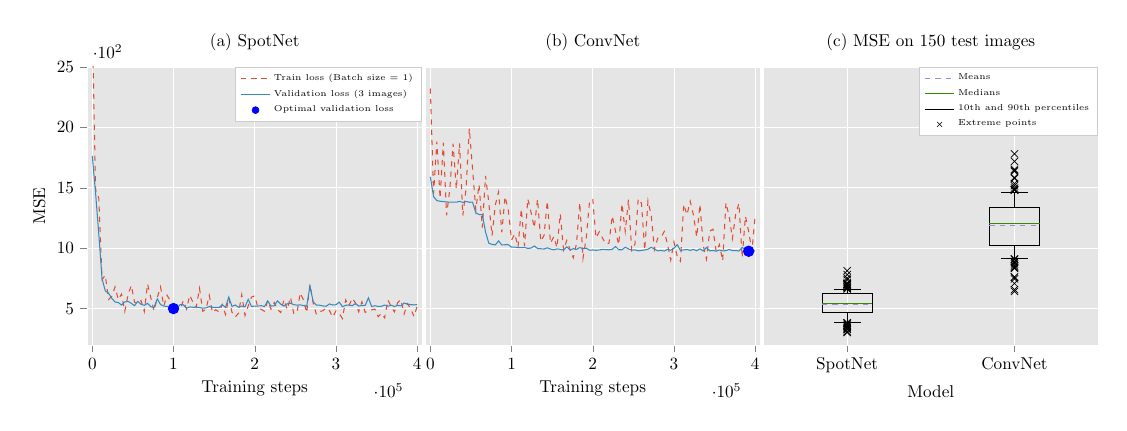
\begin{tikzpicture}[scale=0.62]

\definecolor{color0}{rgb}{0.886274509803922,0.290196078431373,0.2}
\definecolor{color1}{rgb}{0.203921568627451,0.541176470588235,0.741176470588235}
\definecolor{color0_boxplot}{rgb}{0.203921568627451,0.541176470588235,0}
\definecolor{color1_boxplot}{rgb}{0.596078431372549,0.556862745098039,0.835294117647059}

\begin{groupplot}[group style={group size=3 by 1,horizontal sep=2pt}]
\def\xs{0.6}
\nextgroupplot[
axis background/.style={fill=white!89.80392156862746!black},
axis line style={white},
legend cell align={left},
legend entries={{Train loss (Batch size = 1)},{Validation loss (3 images)},{Optimal validation loss}},
legend style={draw=white!80.0!black,at={(1,1)},font=\tiny},
tick align=outside,
tick pos=left,
title={(a) SpotNet },
x grid style={white},
xlabel={Training steps},
xmajorgrids,
xmin=-6000, xmax=406000,
y grid style={white},
ylabel={MSE},
ymajorgrids,
ymin=200, ymax=2500,
scaled y ticks = base 10:-2,
]
\addlegendimage{no markers,dashed, color0}
\addlegendimage{no markers, color1}
\addlegendimage{only marks, blue}
\addplot [semithick, color0,dashed]
table [row sep=\\]{%
0	2873.9402 \\
4000	1487.4771 \\
8000	1412.4348 \\
12000	740.2077 \\
16000	776.4274 \\
20000	575.8815 \\
24000	600.7701 \\
28000	679.447 \\
32000	574.5651 \\
36000	620.2233 \\
40000	477.6323 \\
44000	613.8904 \\
48000	692.6459 \\
52000	553.5771 \\
56000	539.6492 \\
60000	566.993 \\
64000	475.6024 \\
68000	704.62 \\
72000	591.6641 \\
76000	481.6077 \\
80000	591.7721 \\
84000	680.5492 \\
88000	520.9133 \\
92000	611.3196 \\
96000	566.3919 \\
100000	470.15 \\
104000	499.618 \\
108000	490.8047 \\
112000	566.0148 \\
116000	496.596 \\
120000	611.0588 \\
124000	550.7266 \\
128000	511.8644 \\
132000	667.8889 \\
136000	478.38 \\
140000	492.8972 \\
144000	610.1896 \\
148000	466.5913 \\
152000	491.6123 \\
156000	471.1522 \\
160000	533.4832 \\
164000	452.0575 \\
168000	587.0078 \\
172000	469.8223 \\
176000	430.9051 \\
180000	461.763 \\
184000	615.3948 \\
188000	443.3753 \\
192000	522.3864 \\
196000	594.914 \\
200000	606.0525 \\
204000	505.6756 \\
208000	494.0137 \\
212000	478.3234 \\
216000	564.8928 \\
220000	495.306 \\
224000	551.1133 \\
228000	492.8544 \\
232000	467.7115 \\
236000	574.1427 \\
240000	492.395 \\
244000	594.6695 \\
248000	460.4045 \\
252000	465.0198 \\
256000	630.3141 \\
260000	572.5755 \\
264000	466.1497 \\
268000	698.7587 \\
272000	544.9118 \\
276000	451.4128 \\
280000	474.8607 \\
284000	483.7791 \\
288000	504.588 \\
292000	484.7041 \\
296000	429.5923 \\
300000	480.9927 \\
304000	460.9509 \\
308000	417.9873 \\
312000	572.0123 \\
316000	522.0478 \\
320000	587.0399 \\
324000	547.3517 \\
328000	473.2666 \\
332000	556.9798 \\
336000	468.7995 \\
340000	484.0967 \\
344000	489.5529 \\
348000	495.9683 \\
352000	433.1085 \\
356000	460.8949 \\
360000	422.9543 \\
364000	571.3148 \\
368000	517.5062 \\
372000	472.9068 \\
376000	548.2503 \\
380000	574.8866 \\
384000	456.5393 \\
388000	540.9498 \\
392000	502.5297 \\
396000	435.4561 \\
400000	518.6477 \\
};
\addplot [semithick, color1]
table [row sep=\\]{%
0	1764.2911 \\
4000	1458.5887 \\
8000	1115.2842 \\
12000	747.3366 \\
16000	646.4179 \\
20000	628.2016 \\
24000	585.459 \\
28000	554.5534 \\
32000	550.4071 \\
36000	529.6862 \\
40000	555.011 \\
44000	560.0368 \\
48000	543.8985 \\
52000	524.5923 \\
56000	560.2757 \\
60000	535.8026 \\
64000	527.082 \\
68000	543.6267 \\
72000	515.3741 \\
76000	509.5202 \\
80000	580.832 \\
84000	533.9949 \\
88000	520.6276 \\
92000	517.8982 \\
96000	516.8859 \\
100000	500.4317 \\
104000	502.1246 \\
108000	532.4986 \\
112000	531.921 \\
116000	503.468 \\
120000	514.3683 \\
124000	511.0636 \\
128000	511.9212 \\
132000	508.8251 \\
136000	503.6625 \\
140000	505.7209 \\
144000	517.6505 \\
148000	510.7726 \\
152000	510.6451 \\
156000	508.4882 \\
160000	532.5638 \\
164000	509.9372 \\
168000	595.9436 \\
172000	517.633 \\
176000	530.1893 \\
180000	511.6764 \\
184000	521.0755 \\
188000	515.0121 \\
192000	576.3154 \\
196000	518.4007 \\
200000	521.3384 \\
204000	521.0539 \\
208000	524.6292 \\
212000	517.0313 \\
216000	564.6754 \\
220000	521.2833 \\
224000	522.9385 \\
228000	563.7763 \\
232000	536.796 \\
236000	521.1968 \\
240000	539.9824 \\
244000	544.8685 \\
248000	533.0778 \\
252000	528.5714 \\
256000	531.1331 \\
260000	524.9901 \\
264000	519.3237 \\
268000	686.5729 \\
272000	557.5596 \\
276000	529.9697 \\
280000	528.0531 \\
284000	522.2173 \\
288000	519.5966 \\
292000	539.0149 \\
296000	530.0518 \\
300000	532.1358 \\
304000	553.6455 \\
308000	516.0965 \\
312000	527.2836 \\
316000	530.3615 \\
320000	524.1199 \\
324000	541.8366 \\
328000	521.5843 \\
332000	525.6605 \\
336000	526.1867 \\
340000	588.9404 \\
344000	516.5328 \\
348000	523.9285 \\
352000	518.058 \\
356000	519.7037 \\
360000	529.5615 \\
364000	520.1326 \\
368000	527.3938 \\
372000	518.0629 \\
376000	526.7527 \\
380000	522.5662 \\
384000	546.1548 \\
388000	538.9417 \\
392000	533.5225 \\
396000	530.8089 \\
400000	533.3585 \\
};
\addplot [semithick, blue, mark=*, mark size=3, mark options={solid}, only marks]
table [row sep=\\]{%
100000	500.4317 \\
};
\nextgroupplot[
axis background/.style={fill=white!89.80392156862746!black},
axis line style={white},
tick align=outside,
tick pos=left,
title={(b) ConvNet },
x grid style={white},
xlabel={Training steps},
xmajorgrids,
xmin=-6000, xmax=406000,
y grid style={white},
ylabel={},
ymajorgrids,
ymin=200, ymax=2500,
scaled y ticks = base 10:-2,
ymajorticks = false,
]
\addplot [semithick, color0,dashed]
table [row sep=\\]{%
0	2321.3057 \\
4000	1452.4852 \\
8000	1881.9786 \\
12000	1413.0874 \\
16000	1872.7573 \\
20000	1272.5352 \\
24000	1489.3918 \\
28000	1863.9 \\
32000	1489.6536 \\
36000	1866.9066 \\
40000	1270.8966 \\
44000	1493.2151 \\
48000	1989.5453 \\
52000	1655.5103 \\
56000	1317.4935 \\
60000	1527.6094 \\
64000	1171.3572 \\
68000	1598.8911 \\
72000	1376.3573 \\
76000	1103.0494 \\
80000	1358.0425 \\
84000	1464.6305 \\
88000	1131.7362 \\
92000	1427.6304 \\
96000	1314.9944 \\
100000	1067.6622 \\
104000	1118.1652 \\
108000	1009.1857 \\
112000	1325.9093 \\
116000	1018.2363 \\
120000	1408.2792 \\
124000	1296.8856 \\
128000	1169.4192 \\
132000	1407.137 \\
136000	1057.1263 \\
140000	1105.0287 \\
144000	1390.3242 \\
148000	1041.9705 \\
152000	1095.2675 \\
156000	1004.6012 \\
160000	1284.1036 \\
164000	985.527 \\
168000	1064.0646 \\
172000	990.3528 \\
176000	920.4621 \\
180000	1038.8396 \\
184000	1377.0148 \\
188000	916.6488 \\
192000	1087.4929 \\
196000	1384.0037 \\
200000	1407.0045 \\
204000	1084.9614 \\
208000	1136.095 \\
212000	1084.1869 \\
216000	1034.7827 \\
220000	1041.6223 \\
224000	1268.0579 \\
228000	1139.8883 \\
232000	1028.5054 \\
236000	1368.162 \\
240000	1139.2946 \\
244000	1402.379 \\
248000	980.7451 \\
252000	1035.1549 \\
256000	1410.1461 \\
260000	1371.791 \\
264000	984.6527 \\
268000	1392.6896 \\
272000	1269.2466 \\
276000	988.5262 \\
280000	1083.4633 \\
284000	1087.4559 \\
288000	1138.2474 \\
292000	1035.1 \\
296000	900.7518 \\
300000	1051.7599 \\
304000	932.1952 \\
308000	891.1969 \\
312000	1363.0844 \\
316000	1275.847 \\
320000	1388.2933 \\
324000	1273.9095 \\
328000	1092.0314 \\
332000	1363.8644 \\
336000	1023.0265 \\
340000	908.9329 \\
344000	1141.1687 \\
348000	1157.1334 \\
352000	971.8505 \\
356000	1030.1417 \\
360000	895.2697 \\
364000	1376.6743 \\
368000	1261.9673 \\
372000	1080.3176 \\
376000	1281.9993 \\
380000	1371.2188 \\
384000	921.4305 \\
388000	1265.0707 \\
392000	1138.5031 \\
396000	976.4579 \\
400000	1270.8306 \\
};
\addplot [semithick, color1]
table [row sep=\\]{%
0	1590.5524 \\
4000	1426.8415 \\
8000	1394.3916 \\
12000	1388.3988 \\
16000	1385.814 \\
20000	1382.8471 \\
24000	1381.1123 \\
28000	1380.4369 \\
32000	1380.3583 \\
36000	1387.4642 \\
40000	1378.5295 \\
44000	1386.9553 \\
48000	1379.9991 \\
52000	1380.7638 \\
56000	1293.2635 \\
60000	1278.1179 \\
64000	1277.674 \\
68000	1133.9457 \\
72000	1040.7609 \\
76000	1031.859 \\
80000	1027.0955 \\
84000	1060.4536 \\
88000	1026.555 \\
92000	1028.4776 \\
96000	1028.8957 \\
100000	1008.2988 \\
104000	1009.2066 \\
108000	1004.2726 \\
112000	1003.9886 \\
116000	1006.257 \\
120000	998.2184 \\
124000	1000.8432 \\
128000	1018.6312 \\
132000	997.6457 \\
136000	995.3231 \\
140000	992.9384 \\
144000	1002.941 \\
148000	992.8294 \\
152000	985.7089 \\
156000	994.3376 \\
160000	990.7282 \\
164000	983.251 \\
168000	1011.4656 \\
172000	984.8436 \\
176000	996.3977 \\
180000	990.302 \\
184000	1004.9018 \\
188000	995.6585 \\
192000	999.9535 \\
196000	983.0239 \\
200000	985.2688 \\
204000	982.321 \\
208000	985.4192 \\
212000	990.2749 \\
216000	988.3309 \\
220000	986.6673 \\
224000	990.6945 \\
228000	1013.7863 \\
232000	987.0336 \\
236000	987.1572 \\
240000	1007.5775 \\
244000	993.8728 \\
248000	983.8595 \\
252000	985.4783 \\
256000	978.2589 \\
260000	981.6657 \\
264000	985.0247 \\
268000	991.5236 \\
272000	1007.33 \\
276000	992.6923 \\
280000	977.7537 \\
284000	981.3038 \\
288000	975.798 \\
292000	990.1171 \\
296000	983.4026 \\
300000	1000.1262 \\
304000	1028.9119 \\
308000	980.9376 \\
312000	985.6753 \\
316000	989.2797 \\
320000	981.6227 \\
324000	989.6844 \\
328000	979.0125 \\
332000	994.3871 \\
336000	976.5054 \\
340000	1006.0644 \\
344000	978.142 \\
348000	980.4649 \\
352000	975.1649 \\
356000	984.6429 \\
360000	978.1816 \\
364000	979.2205 \\
368000	989.5524 \\
372000	980.1757 \\
376000	980.3916 \\
380000	976.1876 \\
384000	1006.7783 \\
388000	984.6764 \\
392000	974.7727 \\
396000	975.4981 \\
400000	978.7233 \\
};
\addplot [semithick, blue, mark=*, mark size=3, mark options={solid}, only marks]
table [row sep=\\]{%
392000	974.7727 \\
};
\nextgroupplot[
axis background/.style = {fill=white!89.80392156862746!black},
axis line style = {white},
tick align = outside,
ytick pos = right, 
xtick pos = left,
yticklabel pos = right,
title={(c) MSE on $150$ test images},
x grid style={white},
xmajorgrids,
xmin=0.5, xmax=2.5,
xminorgrids,
xtick={1,2},
xticklabels={SpotNet,ConvNet},
xlabel = {Model},
y grid style={white},
ymajorticks = false,
ymajorgrids,
ymin=200, ymax=2500,
yminorgrids,
scaled y ticks = base 10:-2,
legend cell align={left},
legend entries={{Means},{Medians},{$10$th and $90$th percentiles},{Extreme points}},
legend style={draw=white!80.0!black,at={(1,1)},font=\tiny},
]
\addlegendimage{no markers, dashed, color1_boxplot}
\addlegendimage{no markers, color0_boxplot}
\addlegendimage{no markers, black}
\addlegendimage{mark=x,black,only marks}
\addplot [black, forget plot]
table [row sep=\\]{%
0.85	465.537841907406 \\
1.15	465.537841907406 \\
1.15	622.255054139163 \\
0.85	622.255054139163 \\
0.85	465.537841907406 \\
};
\addplot [black, forget plot]
table [row sep=\\]{%
1	465.537841907406 \\
1	386.380992235547 \\
};
\addplot [black, forget plot]
table [row sep=\\]{%
1	622.255054139163 \\
1	662.338396277441 \\
};
\addplot [black, forget plot]
table [row sep=\\]{%
0.92	386.380992235547 \\
1.08	386.380992235547 \\
};
\addplot [black, forget plot]
table [row sep=\\]{%
0.92	662.338396277441 \\
1.08	662.338396277441 \\
};
\addplot [black, mark=x, mark size=3, mark options={solid,fill opacity=0}, only marks, forget plot]
table [row sep=\\]{%
1	371.309487590004 \\
1	344.457311039467 \\
1	327.793108147659 \\
1	341.19264482169 \\
1	383.011632691107 \\
1	329.372469015289 \\
1	355.261977699138 \\
1	301.980405421624 \\
1	355.892736662058 \\
1	309.137028507265 \\
1	379.439406766405 \\
1	332.673260078804 \\
1	381.232917791638 \\
1	361.763225647003 \\
1	308.189498975352 \\
1	683.454480817845 \\
1	714.622127439401 \\
1	677.419387908248 \\
1	692.528502920622 \\
1	704.201920589072 \\
1	813.005530759816 \\
1	662.695667833273 \\
1	704.422107318418 \\
1	669.392690389817 \\
1	781.26531735278 \\
1	738.398542913141 \\
1	694.799352773159 \\
1	752.395691566497 \\
1	676.997852732728 \\
1	702.913873300358 \\
};
\addplot [black, forget plot]
table [row sep=\\]{%
1.85	1025.439631143 \\
2.15	1025.439631143 \\
2.15	1334.44458031024 \\
1.85	1334.44458031024 \\
1.85	1025.439631143 \\
};
\addplot [black, forget plot]
table [row sep=\\]{%
2	1025.439631143 \\
2	915.868842679265 \\
};
\addplot [black, forget plot]
table [row sep=\\]{%
2	1334.44458031024 \\
2	1463.01855796749 \\
};
\addplot [black, forget plot]
table [row sep=\\]{%
1.92	915.868842679265 \\
2.08	915.868842679265 \\
};
\addplot [black, forget plot]
table [row sep=\\]{%
1.92	1463.01855796749 \\
2.08	1463.01855796749 \\
};
\addplot [black, mark=x, mark size=3, mark options={solid,fill opacity=0}, only marks, forget plot]
table [row sep=\\]{%
2	853.919341625797 \\
2	843.183706965714 \\
2	707.963215350935 \\
2	746.21227340565 \\
2	837.356577657166 \\
2	761.179238857815 \\
2	656.879010956964 \\
2	832.227028534921 \\
2	882.843486074756 \\
2	761.209548885781 \\
2	890.56629302798 \\
2	643.102642785651 \\
2	870.026690307455 \\
2	911.28209140513 \\
2	907.837023636585 \\
2	2254.6270777611 \\
2	1483.22405437115 \\
2	1480.22208527229 \\
2	1636.35661390887 \\
2	1780.41142889174 \\
2	1652.8534597348 \\
2	1482.49452383345 \\
2	1585.23417966965 \\
2	1516.43924310494 \\
2	1484.75195905914 \\
2	1717.78561905625 \\
2	1643.56391539098 \\
2	1533.74206019701 \\
2	1497.3110693821 \\
2	1577.81725203656 \\
};
\addplot [color0_boxplot, forget plot]
table [row sep=\\]{%
0.85	539.969755104348 \\
1.15	539.969755104348 \\
};
\addplot [color1_boxplot, dashed, forget plot]
table [row sep=\\]{%
0.85	538.19854104976 \\
1.15	538.19854104976 \\
};
\addplot [color0_boxplot, forget plot]
table [row sep=\\]{%
1.85	1205.39122641264 \\
2.15	1205.39122641264 \\
};
\addplot [color1_boxplot, dashed, forget plot]
table [row sep=\\]{%
1.85	1189.68665208323 \\
2.15	1189.68665208323 \\
};
\end{groupplot}

\end{tikzpicture}

    \end{center}
    
    \vspace{-10pt}
    
    Explore \href{https://github.com/poldap/SpotNet}{github.com/poldap/SpotNet} to see the generation of these figures in Python.
    
    \vspace{5pt}
    
    {\footnotesize Part of \fullcite{AguilaPla2019}}
\end{frame}

\begin{frame}{Practical TikZ Tutorial - Remarks}
    \begin{itemize}
        \item Use the same styles (fonts, font sizes, math symbols, etc.) across your papers, i.e., in your figures, in your text, etc.
        \item Work only with scalable graphics
        \item Put no limits on the drawing possibilities, promote creativity and clear communication
        \item Re-use drawings and figures, get your time back
        \item Use TikZ :-D
    \end{itemize}
    A word of warning: local compilation will require \texttt{pdflatex -shell-escape} or \texttt{pdflatex --shell-escape} (depending on your \LaTeX distribution) for many of the examples. Compliation time will benefit from the use of \texttt{\textbackslash usetikzlibrary\{external\}} \texttt{\textbackslash tikzexternalize} in the preamble of your document.
\end{frame}

\end{document}
